\documentclass[10pt,english,aspectratio=169]{beamer}

\usepackage{ae,aecompl}
\usepackage[T1]{fontenc}
\usepackage{textcomp}
\usepackage[utf8]{inputenc}
\usepackage{babel}

\setcounter{secnumdepth}{3}
\setcounter{tocdepth}{3}

\usepackage{amsmath, amssymb, graphicx}
\usepackage{booktabs, multirow}
\usepackage{tikz}
\usetikzlibrary{positioning,arrows.meta,shapes,calc,fit,backgrounds}
\usepackage{listings}
\usepackage{xcolor}
\usepackage{tcolorbox}

\lstset{
  basicstyle=\ttfamily\small,
  keywordstyle=\color{blue!80!black}\bfseries,
  commentstyle=\color{green!50!black}\itshape,
  stringstyle=\color{orange!80!black},
  backgroundcolor=\color{gray!8},
  frame=single,
  rulecolor=\color{gray!40},
  breaklines=true,
  showstringspaces=false,
  numbers=none,
}

\lstdefinestyle{pythonstyle}{
    language=Python,
    basicstyle=\ttfamily\footnotesize,
    keywordstyle=\color{blue!80!black}\bfseries,
    commentstyle=\color{green!50!black}\itshape,
    stringstyle=\color{orange!80!black},
    frame=single,
    rulecolor=\color{gray!40},
    backgroundcolor=\color{gray!8},
    breaklines=true,
    showstringspaces=false,
    numbers=left,
    numbersep=5pt,
    numberstyle=\tiny\color{gray}
}

\lstdefinestyle{markdownstyle}{
    basicstyle=\ttfamily\footnotesize,
    frame=single,
    rulecolor=\color{gray!40},
    backgroundcolor=\color{gray!8},
    breaklines=true,
    showstringspaces=false,
    numbers=none,
}

\ifx\hypersetup\undefined
  \AtBeginDocument{%
    \hypersetup{bookmarks=false,breaklinks=true,pdfborder={0 0 0},colorlinks=true,
      linkcolor=DarkText,urlcolor=RedTitle}%
  }
\else
  \hypersetup{bookmarks=false,breaklinks=true,pdfborder={0 0 0},colorlinks=true,
    linkcolor=DarkText,urlcolor=RedTitle}%
\fi

\makeatletter
\AtBeginDocument{%
  \let\origtableofcontents=\tableofcontents
  \def\tableofcontents{\@ifnextchar[{\origtableofcontents}{\gobbletableofcontents}}
  \def\gobbletableofcontents#1{\origtableofcontents}%
}

\usetheme{metropolis}
\metroset{sectionpage=none,subsectionpage=none}
\usefonttheme{professionalfonts}

\definecolor{LightGray}{RGB}{230,230,230}
\definecolor{RedTitle}{RGB}{0,0,200}
\definecolor{VeryLightGray}{RGB}{245,245,245}
\definecolor{DarkText}{RGB}{0,0,0}

\setbeamercolor{background canvas}{bg=white}
\setbeamercolor{title}{fg=RedTitle}
\setbeamercolor{author}{fg=DarkText}
\setbeamercolor{date}{fg=DarkText}
\setbeamercolor{frametitle}{bg=VeryLightGray,fg=DarkText}
\setbeamercolor{normal text}{fg=DarkText}

\setbeamersize{text margin left=5mm, text margin right=5mm}
\addtobeamertemplate{frametitle}{}{\vspace{-0.5em}}
\newcommand{\reducevspace}{\vspace{-0.5cm}}

\setbeamertemplate{navigation symbols}{}
\setbeamertemplate{footline}{%
  \hfill%
  \usebeamercolor[fg]{page number in head/foot}%
  \usebeamerfont{page number in head/foot}%
  \insertframenumber\,/\,\inserttotalframenumber\kern1em\vskip2pt%
}
\makeatother

\graphicspath{{figures/}{Exercise10_ES_Fellows/plots/}}

\newcommand{\sectiondivider}[2]{%
\begin{frame}[plain,noframenumbering]
\begin{center}
\vfill
{\Large\textbf{#1}\par}
\vspace{0.35cm}
{\normalsize #2\par}
\vfill
\end{center}
\end{frame}
}

\title[ML \& Agentic AI for Macro Research]{Machine Learning and Agentic AI for Macroeconomic Research}
\subtitle{Lec.~10: Case Studies --- Agentic AI in Economic Research}
\author{Zhigang Feng}
\date{Spring 2026}

\begin{document}

\begin{frame}[plain]
\begin{center}
\vspace{1.2cm}
{\Large\textbf{Machine Learning and Agentic AI for Macroeconomic Research}\par}
\vspace{0.35cm}
{\large Lec.~10: Case Studies --- Agentic AI in Economic Research\par}
\vspace{0.8cm}
{\normalsize Zhigang Feng\par}
\vspace{0.1cm}
{\normalsize Spring 2026\par}
\end{center}
\end{frame}

\begin{frame}{Lecture Agenda}
\begin{columns}[T]
\begin{column}{0.48\textwidth}
\begin{enumerate}
    \item Why case studies after Lec.~9
    \item Three research patterns
    \item Case Study 1: paper-review skill
    \item Case Study 2: MEPS uninsurance
    \item Case Study 3: ES fellows dataset
    \item Case Study 4: AI as research collaborator
    \item Case Study 5: inside the sprint (process walkthrough)
\end{enumerate}
\end{column}
\begin{column}{0.48\textwidth}
\begin{enumerate}
    \setcounter{enumi}{7}
    \item Synthesis across the cases
    \item Exercise A: guided MEPS lab
    \item Exercise B: fellows assignment
    \item Appendix: prompts, schema, and references
\end{enumerate}
\end{column}
\end{columns}

\vspace{0.3cm}
\textbf{Teaching claim:} agents help economists in three concrete ways ---
reusable quality-control workflows, empirical data pipelines, and provenance-aware public-web dataset construction --- and one meta way: as a full-lifecycle collaborator whose workflow is itself a studied object (Case~5).
\end{frame}

%===========================================================
\section{Framing}
%===========================================================

\sectiondivider{Framing}{From Lec.~9 concepts to complete research workflows}

\begin{frame}{Where We Are in the Course}
\begin{center}
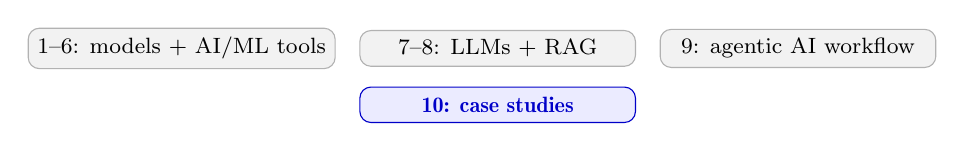
\begin{tikzpicture}[
    node distance=0.25cm,
    lecture/.style={rectangle, rounded corners, draw=gray!60, fill=gray!10,
        minimum width=3.5cm, minimum height=0.45cm, font=\footnotesize, text=DarkText},
    current/.style={rectangle, rounded corners, draw=RedTitle, fill=blue!8,
        minimum width=3.5cm, minimum height=0.45cm, font=\footnotesize\bfseries, text=RedTitle},
]
\node[lecture] (l1) {1--6: models + AI/ML tools};
\node[lecture, right=0.3cm of l1] (l2) {7--8: LLMs + RAG};
\node[lecture, right=0.3cm of l2] (l3) {9: agentic AI workflow};
\node[current, below=0.25cm of l2] (l4) {10: case studies};
\end{tikzpicture}
\end{center}

\vspace{0.3cm}
\begin{itemize}
    \item Lec.~9 gave the workflow: specification, structure, validation, and human oversight
    \item Lec.~10 shows how that workflow changes shape across different research jobs
    \item The core question is no longer ``what is a skill?'' It is ``what workflow should I build for this task?''
\end{itemize}
\end{frame}

\begin{frame}{Lab Readiness Check}

Before today's exercises, verify all five:

\vspace{0.2cm}

\begin{enumerate}
    \item \textbf{Claude Code installed} --- \texttt{claude --version} returns a version number

    \vspace{0.1cm}

    \item \textbf{Subscription active} --- Pro or Max at \texttt{claude.ai}

    \vspace{0.1cm}

    \item \textbf{Git initialized in your project} --- \texttt{git status} runs without error

    \vspace{0.1cm}

    \item \textbf{Working Python or R environment} --- \texttt{which python} or \texttt{which R} returns a path

    \vspace{0.1cm}

    \item \textbf{CLAUDE.md created} --- one file with your project name, language, and goal
\end{enumerate}

\vspace{0.3cm}

\textbf{If any box is unchecked,} open Appendix~A now. The exercises in this lecture require all five. If setup takes more than 10 minutes, pair with a neighbor and share one terminal.
\end{frame}

\begin{frame}{Why Case Studies After Lec.~9}
\begin{itemize}
    \item Knowing the vocabulary of agentic AI does not tell you how to design a research workflow
    \item The difficult step is decomposition: where to split the task, where to validate, and what stays human
    \item Different tasks need different harnesses:
    paper review is not the same as MEPS harmonization, and neither is the same as public-web metadata collection
    \item Today is about design judgment, not product loyalty
\end{itemize}

\vspace{0.35cm}
\textbf{Question for every case:} what is the artifact, what is the failure mode, and what must the economist still verify?
\end{frame}

\begin{frame}{Three Research Patterns}
\small
\begin{tabular}{p{3.0cm}p{4.1cm}p{5.2cm}}
\toprule
\textbf{Pattern} & \textbf{Representative task} & \textbf{Main risk if you use the wrong workflow} \\
\midrule
Reusable skill & Referee-style paper review & Generic comments, hallucinated quotes, missing quality gate \\
Empirical pipeline & MEPS harmonization and figures & Wrong crosswalk, dropped survey weights, silent validation failure \\
Public-web dataset & Econometric Society fellows metadata & Broken source discipline, missing provenance, hidden missingness \\
\bottomrule
\end{tabular}

\vspace{0.3cm}
\textbf{All three use agents, but the harness is different.}
\end{frame}

\begin{frame}{What Remains Human Across All Three}
\begin{columns}[T]
\begin{column}{0.48\textwidth}
\textbf{You still own}
\begin{itemize}
    \item the research question
    \item the coding rules
    \item the validation target
    \item the interpretation
    \item the decision to trust or reject the output
\end{itemize}
\end{column}
\begin{column}{0.48\textwidth}
\textbf{The agent accelerates}
\begin{itemize}
    \item repetitive execution
    \item file handling
    \item promptable decomposition
    \item re-runs after fixes
    \item draft diagnostics and plots
\end{itemize}
\end{column}
\end{columns}

\vspace{0.35cm}
\textbf{Lec.~9 still governs this lecture:} specification and validation are not optional just because the execution is faster.
\end{frame}

%===========================================================
\section{Case Study 1: Paper Review Skill}
%===========================================================

\sectiondivider{Case Study 1}{A reusable quality-control workflow for paper review}

\begin{frame}{Case Study 1: Why This Becomes a Skill}
\begin{tcolorbox}[colback=blue!3, colframe=RedTitle!60]
\textbf{Research job:} produce a structured referee-style review for a quantitative economics paper with quote-level evidence and quality gates.
\end{tcolorbox}

\vspace{0.3cm}
\begin{itemize}
    \item You may run this workflow many times across papers, coauthors, and seminars
    \item Quality matters more than speed because a wrong criticism is costly
    \item The task has internal stages with clear dependencies
    \item That makes it a good candidate for a reusable skill rather than a one-off prompt
\end{itemize}
\end{frame}

\begin{frame}{The Naive Baseline Fails Fast}
\textbf{Tempting prompt:} ``Review this paper.''

\vspace{0.25cm}
\textbf{What usually comes back:}
\begin{itemize}
    \item generic praise and generic weaknesses
    \item no verbatim anchor to the paper
    \item no proof-checking discipline
    \item no calibration to quantitative macro standards
    \item no filter removing low-confidence comments
\end{itemize}

\vspace{0.3cm}
\textbf{The failure is not just model quality.} It is the absence of structure, specialization, and a final editorial gate.
\end{frame}

\begin{frame}[fragile]{What a High-Quality Output Should Look Like}
\begin{tcolorbox}[colback=gray!5, colframe=gray!40, title={\footnotesize Shortened review template}, fonttitle=\bfseries\footnotesize]
\begin{lstlisting}[style=markdownstyle, basicstyle=\ttfamily\scriptsize]
## Overall Feedback
1. Estimand is not fully pinned down in Section 2.3
2. Proof of Theorem 2 needs one missing justification
3. Numerical section needs a reproducibility note

## Detailed Comments
### 1. Proof step in Theorem 2
Quote: "By dominated convergence ..."
Feedback: This step needs an explicit domination argument.
\end{lstlisting}
\end{tcolorbox}

\vspace{0.25cm}
\textbf{Target properties:} issue prioritization, exact anchoring, specific fixes, and a recommendation you can defend.
\end{frame}

\begin{frame}{The 7-Phase Pipeline}
\begin{center}
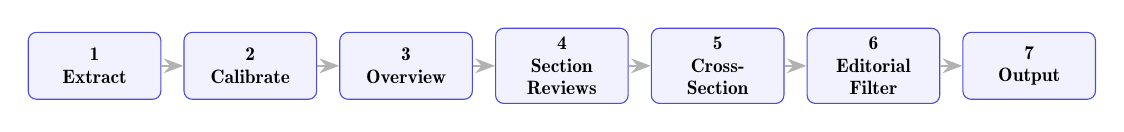
\begin{tikzpicture}[
    phase/.style={rectangle, rounded corners=3pt, draw=RedTitle!70, fill=blue!5,
        minimum width=1.5cm, minimum height=0.85cm, font=\scriptsize\bfseries,
        text width=1.45cm, align=center, text=DarkText},
    arr/.style={-{Stealth[length=2.5mm]}, thick, gray!60},
]
\node[phase] (p1) {1\\Extract};
\node[phase, right=0.28cm of p1] (p2) {2\\Calibrate};
\node[phase, right=0.28cm of p2] (p3) {3\\Overview};
\node[phase, right=0.28cm of p3] (p4) {4\\Section\\Reviews};
\node[phase, right=0.28cm of p4] (p5) {5\\Cross-\\Section};
\node[phase, right=0.28cm of p5] (p6) {6\\Editorial\\Filter};
\node[phase, right=0.28cm of p6] (p7) {7\\Output};

\draw[arr] (p1) -- (p2);
\draw[arr] (p2) -- (p3);
\draw[arr] (p3) -- (p4);
\draw[arr] (p4) -- (p5);
\draw[arr] (p5) -- (p6);
\draw[arr] (p6) -- (p7);
\end{tikzpicture}
\end{center}

\vspace{0.25cm}
\begin{itemize}
    \item Parallelism happens inside phases, not across them
    \item The output of one phase becomes the acceptance criteria for the next
    \item This is a quality-control pipeline, not just a prompt chain
\end{itemize}
\end{frame}

\begin{frame}{Why Decomposition Matters Here}
\begin{columns}[T]
\begin{column}{0.32\textwidth}
\textbf{Context}
\begin{itemize}
    \item long paper
    \item review rules
    \item output template
\end{itemize}
One call is too coarse.
\end{column}
\begin{column}{0.32\textwidth}
\textbf{Specialization}
\begin{itemize}
    \item proof review
    \item methodology review
    \item literature fit
\end{itemize}
One prompt does not do all well.
\end{column}
\begin{column}{0.32\textwidth}
\textbf{Quality}
\begin{itemize}
    \item generic comments
    \item invented quotes
    \item duplicated issues
\end{itemize}
You need a final filter.
\end{column}
\end{columns}

\vspace{0.3cm}
\textbf{Economics translation:} this is like assigning specialized RA tasks, then forcing everything through one senior review before it goes out.
\end{frame}

\begin{frame}{The Highest-Value Guardrails}
\begin{enumerate}
    \item \textbf{Confidence gate.} Do not assert an error unless the model can derive it step by step.
    \item \textbf{Quote verification.} Comments that cite the paper must be anchored to real text.
    \item \textbf{Editorial filter.} Remove generic advice, duplicates, and stylistic fluff.
    \item \textbf{Humanization.} The final report should read like a serious economics referee report, not model boilerplate.
\end{enumerate}

\vspace{0.3cm}
\textbf{The lesson is broader than paper review:} when the stakes are high, validation must be a named stage in the workflow.
\end{frame}

\begin{frame}{Worked Example: Why the MPE Paper Is a Good Stress Test}
\begin{tcolorbox}[colback=blue!3, colframe=RedTitle!60]
\textbf{Demo paper:} \textit{Markov Equilibria with Quasi-Hyperbolic Discounting}
\end{tcolorbox}

\vspace{0.25cm}
\begin{itemize}
    \item it mixes proofs, numerical work, and dynamic economic interpretation
    \item it forces the workflow to separate theorem checking from broader conceptual review
    \item it is hard enough that a one-shot prompt should fail
\end{itemize}

\vspace{0.3cm}
\textbf{This is why case studies matter:} you only learn the workflow once you see where the naive baseline actually breaks.
\end{frame}

\begin{frame}{What the Economist Still Owns in Case Study 1}
\begin{columns}[T]
\begin{column}{0.48\textwidth}
\textbf{Agent side}
\begin{itemize}
    \item parse sections
    \item fan out specialized prompts
    \item draft comments
    \item enforce formatting
\end{itemize}
\end{column}
\begin{column}{0.48\textwidth}
\textbf{Economist side}
\begin{itemize}
    \item decide what counts as a serious objection
    \item reject false positives
    \item judge novelty and importance
    \item decide what feedback is worth sending
\end{itemize}
\end{column}
\end{columns}

\vspace{0.3cm}
\textbf{Skill logic:} you are not outsourcing judgment. You are outsourcing disciplined first-pass execution.
\end{frame}

\begin{frame}{When Should a Workflow Become a Skill?}
\small
\begin{tabular}{p{5.7cm}p{6.0cm}}
\toprule
\textbf{Build a skill when ...} & \textbf{Stay ad hoc when ...} \\
\midrule
you will repeat the workflow many times & the task is one-off \\
the workflow has named validation stages & you are still exploring what the workflow should be \\
multiple users need consistent output & only one user needs the result \\
quality failures are expensive & output format is flexible \\
\bottomrule
\end{tabular}

\vspace{0.3cm}
\textbf{Case 1 verdict:} this is a skill because repeatability and quality control are the point.
\end{frame}

%===========================================================
\section{Case Study 2: MEPS Uninsurance}
%===========================================================

\sectiondivider{Case Study 2}{A one-session empirical data pipeline with strong validation}

\begin{frame}{Case Study 2: The Macro Question}
\begin{tcolorbox}[colback=blue!3, colframe=RedTitle!60]
\textbf{Question:} Who is uninsured in the United States, 2000--2023, and how did the ACA change the distribution?
\end{tcolorbox}

\vspace{0.25cm}
\begin{itemize}
    \item health insurance is a major incomplete-market margin
    \item the ACA is a large social-insurance intervention
    \item the research value comes from who gained coverage, not just from the overall average
    \item this is the most economics-facing case in the lecture
\end{itemize}
\end{frame}

\begin{frame}{The Naive Baseline: 24 Files, 24 Headaches}
\begin{itemize}
    \item download 24 MEPS full-year files by hand
    \item discover that variable names are year-suffixed
    \item figure out which weight variable applies in each year
    \item merge everything and hope the crosswalk is right
\end{itemize}

\vspace{0.3cm}
\textbf{Where this breaks:}
\begin{enumerate}
    \item silent crosswalk mistakes
    \item dropped survey weights
    \item inconsistent file formats
    \item wrong figure even though the code runs
\end{enumerate}
\end{frame}

\begin{frame}{Why This Stays Ad Hoc Instead of Becoming a Skill}
\begin{columns}[T]
\begin{column}{0.48\textwidth}
\textbf{Skill-like features}
\begin{itemize}
    \item multi-step pipeline
    \item explicit validation
    \item repeated checks
\end{itemize}
\end{column}
\begin{column}{0.48\textwidth}
\textbf{Why still ad hoc}
\begin{itemize}
    \item single research question
    \item only three prompts
    \item interactive refinement of plots
    \item workflow is useful but not yet a reusable product
\end{itemize}
\end{column}
\end{columns}

\vspace{0.3cm}
\textbf{Case 2 verdict:} this is a structured session, not a reusable skill.
\end{frame}

\begin{frame}[fragile]{The 3-Prompt Architecture}
\begin{lstlisting}[style=pythonstyle, language={}, basicstyle=\ttfamily\scriptsize, numbers=none]
Prompt A: download, parse, and harmonize MEPS files
Prompt B: compute weighted uninsurance rates by group
Prompt C: generate publication-quality figures and annotations
\end{lstlisting}

\vspace{0.25cm}
\begin{itemize}
    \item Phase A builds infrastructure
    \item Phase B turns infrastructure into statistics
    \item Phase C turns statistics into economic evidence
\end{itemize}
\end{frame}

\begin{frame}{Phase A: What the Agent Actually Does}
\begin{itemize}
    \item discovers the AHRQ download pattern
    \item retries around 403 or parser failures
    \item builds a year-specific crosswalk
    \item standardizes the merged output into one panel
\end{itemize}

\vspace{0.25cm}
\textbf{This is the boring but decisive part.} If the infrastructure is wrong, every figure downstream is wrong in a disciplined-looking way.
\end{frame}

\begin{frame}{Schema Harmonization Is the Hard Part}
\small
\begin{tabular}{lccc}
\toprule
\textbf{Concept} & \textbf{2001} & \textbf{2014} & \textbf{2022} \\
\midrule
Insurance coverage & \texttt{INSCOV01} & \texttt{INSCOV14} & \texttt{INSCOV22} \\
Person weight & \texttt{PERWT01F} & \texttt{PERWT14F} & \texttt{PERWT22F} \\
Age & year-specific & \texttt{AGELAST} & \texttt{AGELAST} \\
\bottomrule
\end{tabular}

\vspace{0.3cm}
\begin{itemize}
    \item humans get tired and miss one mapping
    \item agents are good at repetitive lookups if you force them to save the crosswalk
    \item validation is still essential because a bad crosswalk can look plausible
\end{itemize}
\end{frame}

\begin{frame}{Weights Are Not Optional}
\[
\text{Uninsurance rate} =
\frac{\sum_i w_i \cdot \mathbf{1}[\texttt{INSCOV}_i = 3]}
{\sum_i w_i}
\]

\vspace{0.25cm}
\begin{itemize}
    \item MEPS is a complex survey, not a simple random sample
    \item unweighted rates distort the national picture
    \item the prompt must state the weighting rule, and you must still inspect the code
\end{itemize}

\vspace{0.25cm}
\textbf{Case 2 lesson:} a fast agent does not relieve you of basic survey-design discipline.
\end{frame}

\begin{frame}{Validation: Trust But Verify}
\small
\begin{tabular}{lcc}
\toprule
\textbf{Year} & \textbf{External benchmark} & \textbf{What your MEPS output should show} \\
\midrule
2010 & CPS ASEC about 16\% & high pre-ACA uninsurance \\
2013 & CPS ASEC 13.4\% & near the pre-ACA peak \\
2016 & CPS ASEC 8.8\% & clear post-2014 decline \\
2019 & CPS ASEC about 8\% & stable late-2010s level \\
2022 & CPS ASEC about 8\% & still low relative to 2000s \\
\bottomrule
\end{tabular}

\vspace{0.3cm}
\textbf{The economist's job:} know enough about the data that a 5\% or 25\% result for 2013 looks obviously wrong.
\end{frame}

\begin{frame}{Figure 1: Overall Uninsurance Rate, 2000--2023}
\begin{center}

\includegraphics[height=0.58\textheight]{fig_overall_uninsurance.pdf}
\end{center}

\vspace{0.1cm}
\textbf{Headline:} high through the 2000s, then a sharp decline after the 2014 ACA coverage expansion.
\end{frame}

\begin{frame}{Figure 2: By Age Group}
\begin{center}

\includegraphics[height=0.58\textheight]{fig_uninsurance_by_age.pdf}
\end{center}

\vspace{0.1cm}
\textbf{Economic reading:} the life-cycle profile is steep, and the post-ACA drop is not uniform across ages.
\end{frame}

\begin{frame}{Figure 3: By Poverty Category}
\begin{center}

\includegraphics[height=0.57\textheight]{fig_uninsurance_by_poverty.pdf}
\end{center}

\vspace{0.1cm}
\textbf{Economic reading:} the largest levels and some of the largest gains are concentrated lower in the income distribution.
\end{frame}

\begin{frame}{Figure 4: By Race and Ethnicity}
\begin{center}

\includegraphics[height=0.58\textheight]{fig_uninsurance_by_race.pdf}
\end{center}

\vspace{0.1cm}
\textbf{Economic reading:} the ACA compresses disparities, but it does not erase them.
\end{frame}

\begin{frame}{Figures 5 and 6: Employment and Region}
\begin{columns}[T]
\begin{column}{0.49\textwidth}

\includegraphics[width=\textwidth]{fig_uninsurance_by_employment.pdf}
\end{column}
\begin{column}{0.49\textwidth}

\includegraphics[width=\textwidth]{fig_uninsurance_heatmap.pdf}
\end{column}
\end{columns}

\vspace{0.15cm}
\textbf{Takeaway:} one pipeline can generate multiple cuts of the same policy story once the harmonized panel exists.
\end{frame}

\begin{frame}{What Claude Did vs.\ What Stayed Human}
\begin{columns}[T]
\begin{column}{0.48\textwidth}
\textbf{Agent}
\begin{itemize}
    \item downloaded files
    \item handled parsing obstacles
    \item built the crosswalk
    \item computed weighted statistics
    \item rendered figures
\end{itemize}
\end{column}
\begin{column}{0.48\textwidth}
\textbf{Economist}
\begin{itemize}
    \item chose the question
    \item specified the weights
    \item chose the subgroup cuts
    \item validated against benchmarks
    \item interpreted the policy story
\end{itemize}
\end{column}
\end{columns}
\end{frame}

\begin{frame}{Exercise A: Guided MEPS Lab}
\begin{itemize}
    \item keep the in-class lab short and structured
    \item students run the same three-prompt arc from the lecture
    \item success criteria:
    one merged file, weighted group-level CSVs, and at least three validated figures
    \item the notebook is the operational handout; the slides only carry the logic
\end{itemize}

\vspace{0.3cm}
\textbf{Pedagogical point:} the lab is about directing the agent and checking the output, not about typing code by hand.
\end{frame}

%===========================================================
\section{Case Study 3: ES Fellows Dataset}
%===========================================================

\sectiondivider{Case Study 3}{A provenance-aware public-web dataset construction workflow}

\begin{frame}{Why This Third Case Is Different}
\begin{itemize}
    \item the source material is public and semi-structured
    \item metadata quality is uneven across people and institutions
    \item missingness is part of the result, not a nuisance to hide
    \item the workflow must control sources, provenance, and coding rules
\end{itemize}

\vspace{0.3cm}
\textbf{This is not a web-scraping stunt.} It is a data-construction problem with explicit source restrictions.
\end{frame}

\begin{frame}{Research Question for the Fellows Dataset}
\begin{tcolorbox}[colback=blue!3, colframe=RedTitle!60]
\textbf{Question:} What can we learn about career stage, election timing, and field composition among current Econometric Society fellows using only official and institutional sources?
\end{tcolorbox}

\vspace{0.25cm}
\begin{itemize}
    \item it is a useful dataset about the economics profession itself
    \item it exposes a new research pattern: roster seed + metadata enrichment + coverage reporting
    \item it forces us to separate current biological age, years since PhD, and age at fellow election
    \item it forces students to confront missingness, source quality, and coding judgment
\end{itemize}
\end{frame}

\begin{frame}{Why a Naive Web-Chat Workflow Still Fails Here}
\begin{enumerate}
    \item \textbf{Roster control is weak.} You need a canonical seed list and fixed batches.
    \item \textbf{Source discipline is weak.} You need a rule that excludes Wikipedia and open-web guesswork.
    \item \textbf{State tracking is weak.} You need persistent files recording what was found and what stayed missing.
    \item \textbf{Auditability is weak.} You need field-level source URLs, not just narrative answers.
\end{enumerate}

\vspace{0.25cm}
\textbf{Precise contrast:} modern web chat can browse and summarize, but this assignment needs a project harness with files, batching, and provenance rules.
\end{frame}

\begin{frame}{Official Seed Roster as of April 14, 2026}
\begin{itemize}
    \item canonical source: the official Econometric Society current fellows page
    \item parsed roster size: 882 fellows
    \item official CV links on the seed page: 64
    \item usable election years in the current page: 880; two entries parse as \texttt{0000}
    \item batching rule: 18 batches of 50 fellows
    \item seed fields: name, affiliation, election year, profile URL, CV URL
\end{itemize}

\vspace{0.25cm}
\textbf{Interpretation:}
\begin{itemize}
    \item the roster is large enough that the workflow must be batched
    \item CV coverage is sparse enough that missingness will remain visible
    \item the current roster is not the same thing as a confirmed-living roster
\end{itemize}
\end{frame}

\begin{frame}{Batch Workflow and Project Structure}
\begin{columns}[T]
\begin{column}{0.48\textwidth}
\textbf{Project files}
\begin{itemize}
    \item seed roster CSV
    \item batch assignment file
    \item normalized batch CSV
    \item analysis script
    \item plots and memo
\end{itemize}
\end{column}
\begin{column}{0.48\textwidth}
\textbf{Workflow}
\begin{enumerate}
    \item parse the official roster
    \item assign a batch of 50
    \item fill official/institutional metadata
    \item run analysis
    \item write findings and limitations
\end{enumerate}
\end{column}
\end{columns}

\vspace{0.3cm}
\textbf{This is the public-web analog of `CLAUDE.md`:} the project files hold the rules and state across sessions.
\end{frame}

\begin{frame}{Schema and Provenance Rules}
\small
\begin{tabular}{p{3.4cm}p{8.4cm}}
\toprule
\textbf{Field} & \textbf{Rule} \\
\midrule
\texttt{name}, \texttt{affiliation}, \texttt{election\_year} & seed roster only \\
\texttt{bio\_url}, \texttt{cv\_url} & official or institutional only \\
\texttt{phd\_year}, \texttt{research\_fields\_raw} & record source URL for each field \\
normalized field bucket & map raw text into the lecture taxonomy \\
\texttt{coverage\_status} & say what remains missing \\
\texttt{notes} & document coding judgment or ambiguity \\
\bottomrule
\end{tabular}

\vspace{0.3cm}
\textbf{Credibility requires traceable provenance for each field.}
\end{frame}

\begin{frame}{Missingness, Gender, and Living-Status Caution}
\begin{itemize}
    \item \textbf{Birth date:} leave missing unless the official source states it
    \item \textbf{PhD year:} use only if the source states the degree year directly
    \item \textbf{Gender:} code only from explicit pronouns or explicit gender language
    \item \textbf{No inference:} not from names, photos, or country
    \item \textbf{Living status:} do not infer from old election year alone; for lecture purposes, use a 90-year cap only as a conservative sensitivity rule
\end{itemize}

\vspace{0.3cm}
\textbf{This is deliberate.} The assignment is designed to teach credible coding rules, not aggressive completion.
\end{frame}

\begin{frame}{Instructor Full Scan: What the Agentic Workflow Added}
\begin{columns}[T]
\begin{column}{0.44\textwidth}
\small
\begin{tabular}{lc}
\toprule
\textbf{Metric} & \textbf{Official $\rightarrow$ Web} \\
\midrule
Local CV docs & 62 $\rightarrow$ 316 \\
Birth year & 11 $\rightarrow$ 46 \\
PhD year & 47 $\rightarrow$ 183 \\
Field bucket & 15 $\rightarrow$ 73 \\
\bottomrule
\end{tabular}

\vspace{0.25cm}
\textbf{Main implication:}
\begin{itemize}
    \item the agent scaled discovery and parsing well
    \item PhD-year coverage improved materially
    \item birth-year coverage stayed thin
\end{itemize}
\end{column}
\begin{column}{0.54\textwidth}
\includegraphics[width=\textwidth]{full_web_coverage_dashboard.pdf}
\end{column}
\end{columns}
\end{frame}

\begin{frame}{The 90-Year Rule Does Not Solve the Main Problem}
\begin{columns}[T]
\begin{column}{0.55\textwidth}
\includegraphics[width=\textwidth]{full_web_age90_status.pdf}
\end{column}
\begin{column}{0.41\textwidth}
\small
\begin{itemize}
    \item observed age $\leq 90$: 44 fellows
    \item observed age $> 90$: 1 fellow
    \item birth year unknown: 836 fellows
\end{itemize}

\vspace{0.2cm}
\textbf{Takeaway:}
\begin{itemize}
    \item the problem is missing birth year, not a handful of extreme ages
    \item do not treat current biological age as the main variable
    \item use age at election or years since PhD instead
\end{itemize}
\end{column}
\end{columns}
\end{frame}

\begin{frame}{Career Stage: Use Years Since PhD and Age at Election}
\begin{columns}[T]
\begin{column}{0.5\textwidth}
\includegraphics[width=\textwidth]{full_web_years_since_phd.pdf}
\end{column}
\begin{column}{0.5\textwidth}
\includegraphics[width=\textwidth]{full_web_age_at_election.pdf}
\end{column}
\end{columns}

\vspace{0.15cm}
\textbf{Main descriptive findings:}
\begin{itemize}
    \item median years since PhD: 35
    \item median age at fellow election: 40
    \item median years from PhD to election: 17
    \item age at election is cleaner than current age because it does not depend on fellows being alive today
    \item this is exactly why agent-generated datasets still need variable-design judgment
\end{itemize}
\end{frame}

\begin{frame}{Election Counts Around Major Economics Events}
\begin{columns}[T]
\begin{column}{0.58\textwidth}
\includegraphics[width=\textwidth]{full_web_event_windows.pdf}
\end{column}
\begin{column}{0.38\textwidth}
\scriptsize
\textbf{3-year post-event windows}
\begin{itemize}
    \item Internet turn (2000): 41 $\rightarrow$ 45
    \item GFC (2008): 35 $\rightarrow$ 51
    \item COVID era (2020): 82 $\rightarrow$ 117
\end{itemize}

\vspace{0.2cm}
\textbf{Interpretation:}
\begin{itemize}
    \item there is no obvious post-dot-com collapse
    \item counts rise after 2008 and surge after 2020
    \item the 2020--2024 jump likely reflects Society-side policy or catch-up effects
    \item use this as descriptive timing evidence, not a causal event study
\end{itemize}
\end{column}
\end{columns}
\end{frame}

\begin{frame}{What Agentic AI Actually Did Here}
\begin{itemize}
    \item discovered and cached candidate homepages at scale, then kept the search state on disk
    \item parsed 527 institutional profile pages and downloaded 316 CV or CV-like documents
    \item normalized fields, tracked source URLs, and reran the analysis after rule changes
    \item surfaced a negative result clearly: even a large search pass does not rescue current biological age
\end{itemize}

\vspace{0.25cm}
\textbf{What stayed human:}
\begin{itemize}
    \item define source restrictions and coding rules
    \item separate current age, years since PhD, and age at election
    \item treat event patterns as descriptive rather than causal
    \item decide when missingness is too severe for a claim
\end{itemize}
\end{frame}

\begin{frame}{Exercise B: Full-Roster Fellows Assignment}
\begin{itemize}
    \item start from the official seed roster and take one batch of 50 fellows
    \item use only official and institutional sources
    \item produce a normalized CSV, four figures, and a short memo
    \item keep missing values visible and documented
    \item use age only if birth-year coverage reaches the lecture threshold; otherwise use years since PhD or age at election
    \item explain clearly what the agent automated and what judgment you supplied
\end{itemize}

\vspace{0.3cm}
\textbf{This case is not about scraping harder.} It is about designing a trustworthy public-web research pipeline.
\end{frame}

%===========================================================
\section{Case Study 4: AI as Research Collaborator}
%===========================================================

\sectiondivider{Case Study 4}{AI as full-lifecycle research collaborator in empirical macroeconomics}

% ---- CS4-01: The Research Question ----
\begin{frame}{Case 4 --- The Research Question}
\begin{tcolorbox}[colback=blue!3, colframe=RedTitle!60]
\textbf{Question:} Why has rapid AI adoption not produced uniform occupational collapse,
and what role does coordinative labor play in shaping which occupations survive?
\end{tcolorbox}
\vspace{0.3cm}
\begin{itemize}
  \item Paper: ``Glue Work, Task Bundles, and the AI Labor Market'' --- Feng (2026, in progress)
  \item Extends Garicano--Li--Wu (2026) by endogenizing bundle strength via glue labor supply
  \item \textbf{This case covers the full research lifecycle:} theory articulation, empirical pipeline design, adversarial review, and claims discipline --- not just one execution stage
\end{itemize}
\end{frame}

% ---- CS4-02: The Glue Work Hypothesis ----
\begin{frame}{The Glue Work Hypothesis}
\begin{columns}[T]
\begin{column}{0.48\textwidth}
\textbf{What is glue work?}
\begin{itemize}
  \item Coordinative tasks that integrate components without producing a visible standalone output
  \item O*NET examples: coordinating work and activities; scheduling; communicating across silos
  \item Underrewarded: workers capture only $\lambda < 1$ of the social marginal product
  \item When glue erodes, the bundle weakens --- often with a lag before it becomes visible
\end{itemize}
\end{column}
\begin{column}{0.48\textwidth}
\textbf{The 2$\times$2 AI impact matrix}
\vspace{0.2cm}

\small
\begin{tabular}{p{2.0cm}p{1.6cm}p{1.6cm}}
\toprule
 & \textbf{Low AI glue} & \textbf{High AI glue} \\
\midrule
\textbf{High AI prod.} & Restructure & Full disruption \\
\textbf{Low AI prod.} & Stable & Glue erosion \\
\bottomrule
\end{tabular}
\vspace{0.3cm}

\footnotesize{Core prediction: high-AI + high-glue occupations \emph{restructure} rather than collapse.}
\end{column}
\end{columns}
\vspace{0.3cm}
\textbf{The insight was human. The matrix formalization was joint.}
\end{frame}

% ---- CS4-03: Stage 1 --- Theory Building ----
\begin{frame}{Stage 1 --- Theory Building with AI}
\begin{itemize}
  \item Human developed the core insight: endogenize bundle strength through glue labor supply
  \item Claude was asked to:
    \begin{itemize}
      \item Articulate the 2$\times$2 prediction matrix from verbal intuition
      \item Define AI-Easy Glue vs.\ AI-Hard Glue using specific O*NET item codes
      \item Identify the market failure formally ($\lambda < 1$ creates underinvestment equilibrium)
    \end{itemize}
  \item \textbf{AI-Easy Glue} (LLM-susceptible): documenting/recording information, synthesizing knowledge, routine cross-functional reporting
  \item \textbf{AI-Hard Glue} (embodied/relational): building trust, mentoring, navigating ambiguous authority, reading implicit organizational signals
  \item Prompting mode: \textbf{specification-driven} --- ``List O*NET items 4C1--4C3 that qualify as AI-Hard Glue by the following criteria\ldots'' not ``tell me what glue work is''
\end{itemize}
\end{frame}

% ---- CS4-04: Stage 2 --- Empirical Specification ----
\begin{frame}[fragile]{Stage 2 --- Translating Theory into Empirical Specification}
\begin{lstlisting}[style=markdownstyle, basicstyle=\tiny\ttfamily]
## Empirical Specification Prompt

You are translating the following theoretical model into a
testable empirical specification.

THEORY CLAIMS:
- P1: High-glue, high-AI-exposure occupations restructure
  rather than collapse (employment share positive 2019-2024)
- P2: The reallocation margin operates at junior entry
  (age < 30), not incumbent exit

VARIABLE CONSTRUCTION RULES:
- glue_core: mean of O*NET items [4C1.a.2, 4A4.a.1, 4A4.b.1]
  normalized to [0,1] at SOC 2018 level
- ai_exposure: FRS AIOE score, 2023 vintage
- outcome: CPS monthly employment share (seasonally adj.)

FORBIDDEN: do not use occupation-level wage as a glue proxy
without first checking correlation > 0.6 with glue_core.
\end{lstlisting}
\footnotesize
\begin{itemize}
  \item Exact item codes prevent hallucinated variable definitions
  \item A ``FORBIDDEN'' instruction enforces scope before results appear
\end{itemize}
\end{frame}

% ---- CS4-05: Claims Discipline ----
\begin{frame}[fragile]{Claims Discipline --- Setting the Rules Before Seeing Results}
\begin{lstlisting}[style=markdownstyle, basicstyle=\tiny\ttfamily]
## Claims Discipline Specification

BEFORE any data is analyzed, record the following:

ALLOWED CLAIMS (theory-derived, testable):
- P1: Occupations in top quartile of both glue_core and AIOE
  show positive employment share growth 2019--2024
- P2: Entry share (age < 30) declines faster in
  low-glue / high-AI occupations

FORBIDDEN CLAIMS (data-mining temptations to block):
- Any claim about wage effects not pre-specified here
- Any interaction term not listed in the model section
- Any subgroup finding discovered post-estimation

GATE: results memo must cite which allowed claim each
regression speaks to before interpretation proceeds.
\end{lstlisting}
\footnotesize\textbf{This is claims discipline.} It must be set before results appear, not reconstructed after.
It is the empirical analog of pre-registration.
\end{frame}

% ---- CS4-06: Pipeline Architecture ----
\begin{frame}{Stage 3 --- The 11-Script Pipeline Architecture}
\begin{center}
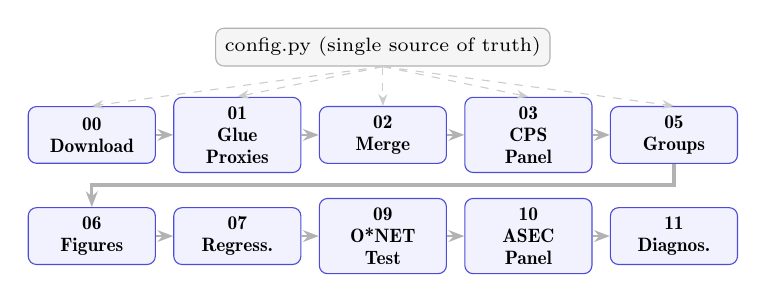
\begin{tikzpicture}[
  pscript/.style={rectangle, rounded corners=3pt, draw=RedTitle!70, fill=blue!5,
    minimum width=1.42cm, minimum height=0.72cm, font=\scriptsize\bfseries,
    text width=1.38cm, align=center},
  cfgnode/.style={rectangle, rounded corners=3pt, draw=gray!60, fill=gray!8,
    minimum width=3.0cm, minimum height=0.48cm, font=\scriptsize, align=center},
  parr/.style={-{Stealth[length=2mm]}, thick, gray!60},
  darr/.style={dashed, gray!40, -{Stealth[length=1.5mm]}},
]
% Top row
\node[pscript] (s00) {00\\Download};
\node[pscript, right=0.22cm of s00] (s01) {01\\Glue\\Proxies};
\node[pscript, right=0.22cm of s01] (s02) {02\\Merge};
\node[pscript, right=0.22cm of s02] (s03) {03\\CPS\\Panel};
\node[pscript, right=0.22cm of s03] (s05) {05\\Groups};
% Config node
\node[cfgnode, above=0.5cm of s02] (cfg) {config.py (single source of truth)};
% Bottom row
\node[pscript, below=0.55cm of s00] (s06) {06\\Figures};
\node[pscript, right=0.22cm of s06] (s07) {07\\Regress.};
\node[pscript, right=0.22cm of s07] (s09) {09\\O*NET\\Test};
\node[pscript, right=0.22cm of s09] (s10) {10\\ASEC\\Panel};
\node[pscript, right=0.22cm of s10] (s11) {11\\Diagnos.};
% Top arrows
\draw[parr] (s00)--(s01); \draw[parr] (s01)--(s02);
\draw[parr] (s02)--(s03); \draw[parr] (s03)--(s05);
% Handoff
\draw[parr, very thick] (s05.south) -- ++(0,-0.27cm) -| (s06.north);
% Bottom arrows
\draw[parr] (s06)--(s07); \draw[parr] (s07)--(s09);
\draw[parr] (s09)--(s10); \draw[parr] (s10)--(s11);
% Config dashes
\foreach \t in {s00,s01,s02,s03,s05}
  \draw[darr] (cfg.south) -- (\t.north);
\end{tikzpicture}
\end{center}
\vspace{0.15cm}
\textbf{One config.py = single source of truth.} \quad 51 unit tests specified before any script runs on real data.
\end{frame}

% ---- CS4-07: Pipeline Module Detail ----
\begin{frame}{Pipeline Module Detail}
\small
\begin{tabular}{p{1.1cm}p{5.6cm}p{5.5cm}}
\toprule
Script & Key output & Validation rule \\
\midrule
00 & onet\_raw, frs\_aioe, crosswalks (parquet) & row count $\geq$ expected; no null SOC codes \\
01 & glue\_proxies (6 variants, SOC 2018) & all variants in $[0,1]$; correlation matrix saved \\
02 & master\_soc: glue + AI exposure + crosswalks & merge rate $\geq 95\%$; no duplicate SOC \\
03 & cps\_panel: employment share, entry share & weights sum to civilian pop; seasonal adj.\ flag set \\
05 & analysis: 4 AI $\times$ glue groups defined & group counts balanced; no SOC in $>1$ group \\
06--11 & figures, tables, diagnostics & files written; no NaN in reported statistics \\
\bottomrule
\end{tabular}
\vspace{0.3cm}
Each script has explicit inputs (parquet), explicit outputs (parquet), and a pass/fail validation rule. Failure halts the pipeline.
\end{frame}

% ---- CS4-08: Variable Construction ----
\begin{frame}{Stage 3 --- Variable Construction Details}
\begin{columns}[T]
\begin{column}{0.46\textwidth}
\textbf{Glue proxies (6 variants)}
\begin{itemize}\small
  \item \texttt{glue\_core}: 3 O*NET items, baseline
  \item \texttt{glue\_ext}: 8-item extended set
  \item \texttt{glue\_aihard}: AI-Hard items only
  \item \texttt{glue\_social}: social/interpersonal subset
  \item \texttt{glue\_dominance}: mean glue / mean all activities
  \item \texttt{glue\_minus\_mgmt}: robustness check
\end{itemize}
\vspace{0.2cm}
\footnotesize{The 6 variants test whether the theory's protection story depends on which aspect of coordination is measured.}
\end{column}
\begin{column}{0.50\textwidth}
\textbf{AI exposure and outcomes}
\begin{itemize}\small
  \item AI exposure: FRS AIOE 2023, SOC-linked
  \item Outcomes: CPS monthly employment share
  \item Entry margin: age $<30$ share within occ-month
  \item Long-run: ASEC panel 2000--2025
  \item 4 groups: median splits of AIOE $\times$ glue\_core
\end{itemize}
\vspace{0.2cm}
\textbf{Core group definitions:}

\small
\begin{tabular}{ll}
High AI + High Glue & Restructuring \\
High AI + Low Glue  & Disruption \\
Low AI + High Glue  & Insulated \\
Low AI + Low Glue   & Stable \\
\end{tabular}
\end{column}
\end{columns}
\end{frame}

% ---- CS4-09: Adversarial Review ----
\begin{frame}{Stage 4 --- Adversarial Review}
\begin{tcolorbox}[colback=blue!3, colframe=RedTitle!60]
\textbf{Adversarial prompt:} ``Find 6 structural weaknesses in this empirical design. For each, state whether it is fatal or manageable, and why.''
\end{tcolorbox}
\vspace{0.2cm}
Six weaknesses identified:
\begin{enumerate}\small
  \item AIOE is cross-sectional --- does not capture within-occupation AI adoption dynamics
  \item Glue proxies are task-level O*NET ratings, not worker-level observations
  \item Selection: high-glue workers may self-select into high-AI firms for unobserved reasons
  \item Crosswalk from SOC 2018 to Census codes loses $\sim$12\% of occupations (a validation rule catches this)
  \item CPS monthly sample sizes for narrow occupations produce large standard errors
  \item \textbf{The interaction (AI $\times$ Glue) is negative in the data} --- but the theory predicts positive
\end{enumerate}
\vspace{0.2cm}
\textbf{Item 6 was the decisive finding.} It repositioned the entire paper.
\end{frame}

% ---- CS4-10: When Data Contradicts Theory ----
\begin{frame}{When Data Contradicts Theory}
\begin{tcolorbox}[colback=blue!3, colframe=RedTitle!60]
\textbf{Data finding:} the estimated interaction (AI exposure $\times$ glue score) is \emph{negative}.\\
\textbf{Theory predicted:} positive --- glue preserves bundles, so high-glue/high-AI should survive.\\
\textbf{This is not a bug.} It is information.
\end{tcolorbox}
\vspace{0.2cm}
\begin{columns}[T]
\begin{column}{0.46\textwidth}
\textbf{What the theory predicted}
\begin{itemize}\small
  \item High-AI + High-Glue $\to$ restructuring and survival
  \item Glue preserves value when production tasks are automated
  \item Expected positive interaction
\end{itemize}
\end{column}
\begin{column}{0.50\textwidth}
\textbf{The reinterpretation}
\begin{itemize}\small
  \item Negative sign: high-glue workers in high-AI occupations are displaced, not preserved
  \item Effect operates through \emph{occupational reallocation}, not within-occupation survival
  \item Theory-specific prediction $\neq$ generic heterogeneity claim
\end{itemize}
\end{column}
\end{columns}
\vspace{0.2cm}
\textbf{Claude distinguished theory-specific predictions from generic heterogeneity findings.} That distinction determines what the paper can claim.
\end{frame}

% ---- CS4-11: Division of Labor ----
\begin{frame}{Division of Labor Across the Full Lifecycle}
\small
\begin{tabular}{p{3.4cm}p{3.2cm}p{5.0cm}}
\toprule
Task & Human Researcher & AI (Claude) \\
\midrule
Core insight & Endogenizes bundle strength via glue & \\
Literature positioning & Sets the GLW extension & \\
Variable specs & Co-designed, approved & Elaborated O*NET codes; caught crosswalk inconsistency \\
Pipeline architecture & Approved the design & Designed 11-script layout from scratch \\
Claims discipline & Enforces the gate & Drafted allowed/forbidden claims \\
Adversarial review & Decided which weaknesses were fatal & Structured the 6 adversarial findings \\
Data execution & Runs the scripts & \\
Interpretation & Final call on repositioning & \\
Paper writing & Authors & Assists with exposition \\
\bottomrule
\end{tabular}
\end{frame}

% ---- CS4-12: Key Prompting Strategies ----
\begin{frame}{Key Prompting Strategies in Case 4}
\begin{enumerate}
  \item \textbf{Specification-driven:} exact O*NET item codes, not vague requests --- prevents hallucinated variable definitions
  \item \textbf{Constraint-based (claims discipline):} allowed and forbidden claims specified before results appear --- prevents data mining
  \item \textbf{Adversarial:} ``find 6 structural weaknesses'' not ``review this memo'' --- prevents sycophantic validation
  \item \textbf{Modular decomposition:} each script as an independent testable unit --- prevents silent errors accumulating across stages
  \item \textbf{Deferred execution:} pipeline fully specified before any real data is analyzed --- separates design from execution, preserving pre-specification discipline
\end{enumerate}
\vspace{0.3cm}
\textbf{Each strategy is a structural response to a specific failure mode, not a stylistic preference.}
\end{frame}

% ---- CS4-13: Failure Modes ----
\begin{frame}{Failure Modes Specific to Case 4}
\begin{enumerate}
  \item \textbf{AI agrees too readily:} asking ``does this design look good?'' produces validation; adversarial mode must be explicit
  \item \textbf{Vague theory $\to$ untestable claims:} ``glue work matters'' is not a prediction; specification-driven prompting forces operationalization
  \item \textbf{Data mining disguised as exploration:} claims discipline must be logged before results; retroactive framing is indistinguishable from pre-specification to a reader
  \item \textbf{Silent crosswalk errors:} the 12\% SOC loss is found only because a validation rule checks merge rate; without validation rules, the pipeline produces credible-looking numbers
  \item \textbf{Mechanical overclaiming:} when data contradicts theory, the temptation is ad hoc reframing; adversarial review forces the repositioning to be deliberate and documented
\end{enumerate}
\end{frame}

% ---- CS4-14: The Meta-Irony ----
\begin{frame}{The Meta-Irony: AI Doing Glue Work}
\begin{columns}[T]
\begin{column}{0.46\textwidth}
\textbf{What the paper studies}
\begin{itemize}
  \item Glue work: coordinative labor that binds complex task bundles
  \item Holds specifications together across stages
  \item Tracks implicit commitments across time
  \item Underrewarded because its contribution is diffuse in output attribution
\end{itemize}
\end{column}
\begin{column}{0.50\textwidth}
\textbf{What Claude did in the research itself}
\begin{itemize}
  \item Maintained specification coherence across 11 scripts and 4 research stages
  \item Tracked which claims were allowed before results arrived
  \item Structured the adversarial review to produce actionable findings
  \item Held the interface between theory and empirical design
\end{itemize}
\end{column}
\end{columns}
\vspace{0.4cm}
\begin{center}
\textbf{The AI is demonstrating its own research subject.}\\
That is not an accident --- it is evidence about where AI comparative advantage lies in complex intellectual work.
\end{center}
\end{frame}

% ---- CS4-15: Key Lessons ----
\begin{frame}{Key Lessons from Case Study 4}
\begin{itemize}
  \item AI can operate across the \textbf{full research lifecycle} --- theory articulation, pipeline design, adversarial review --- not just execution
  \item The human researcher must own the core insight, literature positioning, data execution, and final interpretation
  \item \textbf{Specification-driven and adversarial prompting} are structural defenses against the most common AI failure modes in research settings
  \item \textbf{Claims discipline} must be established before results appear; it cannot be reconstructed credibly after
  \item When data contradicts theory, the right move is deliberate repositioning, not ad hoc reframing; AI can structure that repositioning but cannot decide whether it is intellectually honest
  \item This is a new pattern: \textbf{AI as full-lifecycle research collaborator}, distinct from skill, empirical pipeline, or dataset harness
\end{itemize}
\end{frame}

%===========================================================
\section{Case Study 5: Inside the Sprint}
%===========================================================

\sectiondivider{Case Study 5}{Inside the sprint --- anatomy of an agentic research workflow, April 15--18, 2026}

% ============================================================
% Frame 5.1 --- What Case 5 Adds
% ============================================================
\begin{frame}{What Case 5 Adds to Case 4}
\begin{columns}[T]
\begin{column}{0.48\textwidth}
\textbf{Case 4 showed the product}
\begin{itemize}\small
  \item research question (glue work + AI labor market)
  \item $2\times 2$ hypothesis
  \item 11-script pipeline
  \item adversarial review and repositioning
  \item division of labor across the lifecycle
\end{itemize}
\end{column}
\begin{column}{0.48\textwidth}
\textbf{Case 5 shows the process}
\begin{itemize}\small
  \item how the first prompt is written
  \item how data are chosen and fetched
  \item how results are read and questioned
  \item how one index becomes four, then a distribution
  \item how LLMs themselves generate new data
  \item how each stage closes with a memo and a critique
\end{itemize}
\end{column}
\end{columns}

\vspace{0.25cm}
\begin{tcolorbox}[colback=blue!3,colframe=RedTitle!60]
\textbf{Guiding claim.} Case 4 answers ``what did the collaboration produce?''. Case 5 answers ``how would a student replay it on a different research question?''. \textbf{Four stages, eight weeks, one puzzle.} Stage 1 (Apr 15--18) is the four-day first sprint; Stages 2--4 layer on dispersion, an LLM-labeled sub/assist index, and the refined within-job distribution.
\end{tcolorbox}
\end{frame}

% ============================================================
% Frame 5.2 --- Four-Day Timeline (swim lanes)
% ============================================================
\begin{frame}{The Four-Day Timeline}
\begin{center}
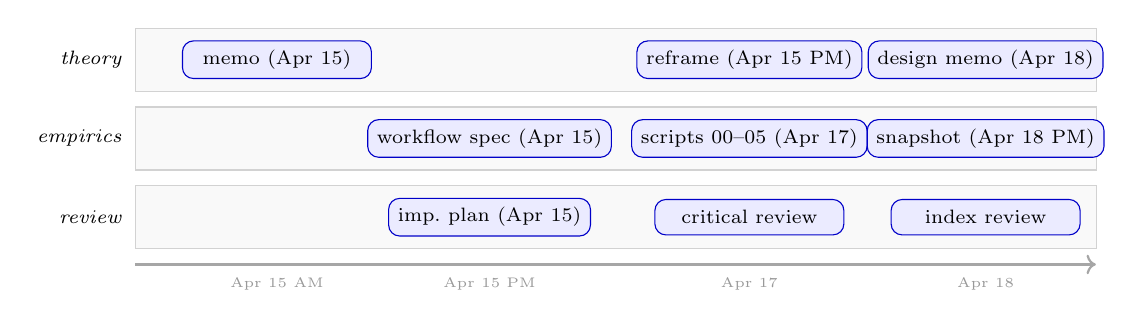
\begin{tikzpicture}[
    node distance=0.1cm,
    act/.style={rectangle, rounded corners, draw=RedTitle, fill=blue!8,
        minimum width=2.4cm, minimum height=0.45cm, font=\scriptsize, text=DarkText, align=center},
    lane/.style={rectangle, draw=gray!35, fill=gray!5,
        minimum width=12.2cm, minimum height=0.8cm, anchor=west, font=\scriptsize},
    lanelabel/.style={font=\scriptsize\itshape, text=DarkText, anchor=east}
]
\node[lane] at (0,2.3) {};
\node[lane] at (0,1.3) {};
\node[lane] at (0,0.3) {};
\node[lanelabel] at ( -0.05, 2.3) {theory};
\node[lanelabel] at ( -0.05, 1.3) {empirics};
\node[lanelabel] at ( -0.05, 0.3) {review};
\node[act] at (1.8, 2.3) {memo (Apr 15)};
\node[act] at (7.8, 2.3) {reframe (Apr 15 PM)};
\node[act] at (10.8, 2.3) {design memo (Apr 18)};
\node[act] at (4.5, 1.3) {workflow spec (Apr 15)};
\node[act] at (7.8, 1.3) {scripts 00--05 (Apr 17)};
\node[act] at (10.8, 1.3) {snapshot (Apr 18 PM)};
\node[act] at (4.5, 0.3) {imp.\ plan (Apr 15)};
\node[act] at (7.8, 0.3) {critical review};
\node[act] at (10.8, 0.3) {index review};
\draw[->, gray!70, thick] (0.0, -0.3) -- (12.2, -0.3);
\node[font=\tiny, gray!80] at (1.8, -0.55) {Apr 15 AM};
\node[font=\tiny, gray!80] at (4.5, -0.55) {Apr 15 PM};
\node[font=\tiny, gray!80] at (7.8, -0.55) {Apr 17};
\node[font=\tiny, gray!80] at (10.8, -0.55) {Apr 18};
\end{tikzpicture}
\end{center}

\vspace{0.15cm}
\textbf{Five acts across three lanes.} 1.~Framing $\to$ 2.~Data strategy $\to$ 3.~Execution $\to$ 4.~Reflection and refinement $\to$ 5.~Writing and iteration. Theory, empirics, and review run in parallel, not in sequence. The next 16 frames walk through these five acts inside Stage 1.
\end{frame}

% ============================================================
% Frame 5.2b --- The Four-Stage Project Arc (NEW)
% ============================================================
\begin{frame}{The Four-Stage Project Arc}
\begin{center}
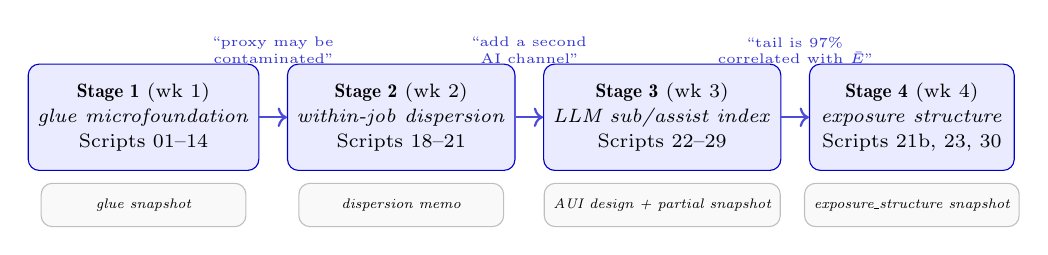
\begin{tikzpicture}[
    node distance=0.35cm,
    stage/.style={rectangle, rounded corners, draw=RedTitle, fill=blue!8,
        minimum width=2.6cm, minimum height=1.35cm, font=\scriptsize, text=DarkText, align=center},
    memo/.style={rectangle, rounded corners, draw=gray!50, fill=gray!5,
        minimum width=2.6cm, minimum height=0.55cm, font=\tiny\itshape, text=DarkText, align=center},
    critique/.style={font=\tiny, text=RedTitle!80, align=center}
]
\node[stage] (s1) {\textbf{Stage 1} (wk 1)\\[1pt]\textit{glue microfoundation}\\[1pt]Scripts 01--14};
\node[stage, right=of s1] (s2) {\textbf{Stage 2} (wk 2)\\[1pt]\textit{within-job dispersion}\\[1pt]Scripts 18--21};
\node[stage, right=of s2] (s3) {\textbf{Stage 3} (wk 3)\\[1pt]\textit{LLM sub/assist index}\\[1pt]Scripts 22--29};
\node[stage, right=of s3] (s4) {\textbf{Stage 4} (wk 4)\\[1pt]\textit{exposure structure}\\[1pt]Scripts 21b, 23, 30};

\node[memo, below=0.15cm of s1] (m1) {glue snapshot};
\node[memo, below=0.15cm of s2] (m2) {dispersion memo};
\node[memo, below=0.15cm of s3] (m3) {AUI design + partial snapshot};
\node[memo, below=0.15cm of s4] (m4) {exposure\_structure snapshot};

\draw[->, RedTitle!70, thick] (s1.east) -- (s2.west);
\draw[->, RedTitle!70, thick] (s2.east) -- (s3.west);
\draw[->, RedTitle!70, thick] (s3.east) -- (s4.west);
\node[critique] at ($(s1.east)!0.5!(s2.west) + (0, 0.85)$) {``proxy may be\\contaminated''};
\node[critique] at ($(s2.east)!0.5!(s3.west) + (0, 0.85)$) {``add a second\\AI channel''};
\node[critique] at ($(s3.east)!0.5!(s4.west) + (0, 0.85)$) {``tail is 97\%\\correlated with \smash{$\bar{E}$}''};
\end{tikzpicture}
\end{center}

\vspace{0.15cm}
\begin{tcolorbox}[colback=blue!3,colframe=RedTitle!60]\scriptsize
\textbf{Pattern.} Each stage ends with a written memo; each transition is a \emph{coauthor-delivered critique} of that memo. Stages are not planned upfront --- each one is scoped from the previous stage's open questions. The workflow is gradual, structured, and human-corrected at every turn.
\end{tcolorbox}
\end{frame}

% ============================================================
% Frame 5.2c --- The Six-Element Stage Template (NEW)
% ============================================================
\begin{frame}{The Six-Element Stage Template}
\begin{columns}[T]
\begin{column}{0.55\textwidth}
\begin{center}
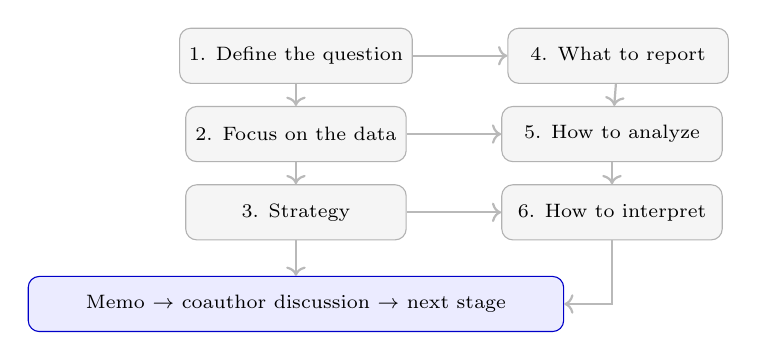
\begin{tikzpicture}[
    node distance=0.28cm,
    elem/.style={rectangle, rounded corners, draw=gray!60, fill=gray!8,
        minimum width=2.8cm, minimum height=0.7cm, font=\scriptsize, text=DarkText, align=center},
    arrow/.style={->, gray!55, thick}
]
\node[elem] (q)     {1. Define the question};
\node[elem, below=of q]     (d) {2. Focus on the data};
\node[elem, below=of d]     (s) {3. Strategy};
\node[elem, right=1.2cm of q] (r) {4. What to report};
\node[elem, right=1.2cm of d] (a) {5. How to analyze};
\node[elem, right=1.2cm of s] (i) {6. How to interpret};
\node[elem, below=0.45cm of s, minimum width=6.8cm, fill=blue!8, draw=RedTitle] (close) {Memo $\to$ coauthor discussion $\to$ next stage};
\draw[arrow] (q) -- (d); \draw[arrow] (d) -- (s);
\draw[arrow] (r) -- (a); \draw[arrow] (a) -- (i);
\draw[arrow] (q.east) -- (r.west); \draw[arrow] (d.east) -- (a.west); \draw[arrow] (s.east) -- (i.west);
\draw[arrow] (s.south) -- (close.north);
\draw[arrow] (i.south) |- (close.east);
\end{tikzpicture}
\end{center}
\end{column}
\begin{column}{0.43\textwidth}
\scriptsize
\textbf{Every stage reuses the same six elements.}
\begin{itemize}\scriptsize
  \item \textbf{Question}: name the specific gap, not the topic.
  \item \textbf{Data}: name the rows and columns, not the dataset.
  \item \textbf{Strategy}: state the identification-\emph{style} claim (descriptive / comparative / causal).
  \item \textbf{Report}: the figures and tables the stage will produce.
  \item \textbf{Analyze}: the spec ladder from simple to preferred.
  \item \textbf{Interpret}: what the result would mean.
\end{itemize}
\vspace{0.15cm}
\begin{tcolorbox}[colback=blue!3,colframe=RedTitle!60]\scriptsize
Stage 1 (next 16 frames) is the detailed walk-through of this template. Stages 2--4 compress it into 4--8 frames each.
\end{tcolorbox}
\end{column}
\end{columns}
\end{frame}

% ============================================================
% Frame 5.3 --- Act 1: Initiating the Discussion
% ============================================================
\begin{frame}{Act 1 --- Initiating the Discussion}
\begin{tcolorbox}[colback=blue!3,colframe=RedTitle!60]
\textbf{Opening prompt.} Open with the \emph{puzzle}, not the method. The first turn names what is unresolved in the field and invites the agent to push back on the framing before any code or measure is mentioned.
\end{tcolorbox}

\vspace{0.2cm}
First-turn material, adapted from \texttt{glue\_work\_research\_memo.md} \S 1:

\begin{tcolorbox}[colback=gray!5,colframe=gray!40]
\footnotesize
Garicano, Li, and Wu (2026) push back on task-level exposure measures by arguing that labor markets price \emph{jobs}, not isolated tasks, so AI affects occupations through a coordination-cost channel. But their coordination cost is exogenous. This memo argues that \textbf{glue work} --- the underrewarded coordination labor that preserves shared context across interdependent tasks --- is the missing microfoundation for bundle strength.
\end{tcolorbox}

\vspace{0.15cm}
\textbf{What the opener buys.} The agent now knows: (i) the paper is theoretical, (ii) the key primitive to be endogenized is coordination cost, (iii) the name of the candidate mechanism is glue work. Everything downstream --- data choice, proxy design, figure set --- is bounded by this frame.
\end{frame}

% ============================================================
% Frame 5.4 --- Theoretical vs Empirical Questions
% ============================================================
\begin{frame}{Defining Theoretical vs.\ Empirical Questions}
\begin{columns}[T]
\begin{column}{0.48\textwidth}
\textbf{Theoretical questions}
\begin{itemize}\small
  \item Can coordination cost $c$ be endogenized as a stock of coordination capital $k$ produced by glue work?
  \item Does $\lambda<1$ (partial appropriation of glue's social value) deliver a welfare externality?
  \item Does a second AI channel $a_g$ acting on coordination tasks weaken bundles that $a_1$ alone would leave intact?
\end{itemize}
\end{column}
\begin{column}{0.48\textwidth}
\textbf{Empirical questions}
\begin{itemize}\small
  \item Do occupations with similar AI exposure but different glue content follow different employment trajectories after November 2022?
  \item Is the divergence stronger for \emph{AI-hard} glue than for coordination in general?
  \item Are AI exposure and glue content empirically orthogonal enough to identify heterogeneity?
\end{itemize}
\end{column}
\end{columns}

\vspace{0.25cm}
\begin{tcolorbox}[colback=blue!3,colframe=RedTitle!60]
\textbf{Discipline.} The two question sets share vocabulary (``bundle strength'', ``coordination'') but not evidence. Theoretical questions are answered by model writing; empirical questions by data. Never let one stand in for the other.
\end{tcolorbox}
\end{frame}

% ============================================================
% Frame 5.5 --- Why Run Empirics First
% ============================================================
\begin{frame}{Why Run the Empirics First}
\begin{itemize}\small
  \item A 62~KB theory memo already existed on Apr 15 21:18. The theory was articulated but not stress-tested.
  \item Empirical illustration is \textbf{cheap to run and expensive to fake}. Running it early exposes any gap between the theory's prediction and what CPS and O*NET actually show.
  \item Journal readers of a theory paper with no motivating evidence do not take the framework seriously. The motivation has to be visible in the first pages.
  \item Case 4's headline lesson --- ``when data contradicts theory, reposition, don't fudge'' --- is only available \emph{because} the empirics ran early enough to contradict anything.
\end{itemize}

\vspace{0.3cm}
\begin{tcolorbox}[colback=blue!3,colframe=RedTitle!60]
\textbf{Ordering rule.} Lead with the empirics whenever the theory is already legible. The empirics act as a first round of adversarial review --- cheaper than a referee and faster than a coauthor.
\end{tcolorbox}
\end{frame}

% ============================================================
% Frame 5.6 --- Sharpening
% ============================================================
\begin{frame}[fragile]{Sharpening --- From ``AI \& Jobs'' to One Window}
\begin{columns}[T]
\begin{column}{0.45\textwidth}
\begin{center}
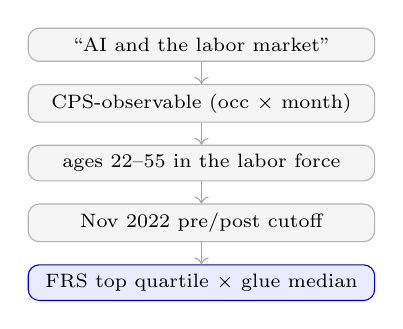
\begin{tikzpicture}[
    node distance=0.28cm,
    box/.style={rectangle, rounded corners, draw=gray!60, fill=gray!8,
        minimum width=4.4cm, minimum height=0.42cm, font=\scriptsize, text=DarkText, align=center},
    final/.style={rectangle, rounded corners, draw=RedTitle, fill=blue!8,
        minimum width=4.4cm, minimum height=0.42cm, font=\scriptsize, text=DarkText, align=center}
]
\node[box] (n1) {``AI and the labor market''};
\node[box, below=of n1] (n2) {CPS-observable (occ $\times$ month)};
\node[box, below=of n2] (n3) {ages 22--55 in the labor force};
\node[box, below=of n3] (n4) {Nov 2022 pre/post cutoff};
\node[final, below=of n4] (n5) {FRS top quartile $\times$ glue median};
\draw[->, gray!70] (n1) -- (n2);
\draw[->, gray!70] (n2) -- (n3);
\draw[->, gray!70] (n3) -- (n4);
\draw[->, gray!70] (n4) -- (n5);
\end{tikzpicture}
\end{center}
\end{column}
\begin{column}{0.55\textwidth}
\textbf{Each narrowing is a decision.}
\begin{itemize}\scriptsize
  \item CPS-observable: rules out within-firm reallocation; only occupational movement is visible.
  \item 22--55: excludes student entry and retirement churn, which move for unrelated reasons.
  \item Nov 2022: coincident with ChatGPT's public release; visible shock, not a causal cutoff.
  \item Top quartile $\times$ median: keeps Group 4 (high-AI, high-glue) large enough to support heterogeneity.
\end{itemize}
\vspace{0.1cm}
\begin{tcolorbox}[colback=gray!5,colframe=gray!40]
\begin{lstlisting}[style=pythonstyle,numbers=none,basicstyle=\ttfamily\scriptsize]
PRE_PERIOD_END      = "2022-10"
POST_PERIOD_START   = "2022-11"
AGE_MAIN            = (22, 55)
MIN_RAW_OBS_PREPOST = 200
AI_HIGH_QUARTILE    = 4
\end{lstlisting}
\end{tcolorbox}
Every narrowing is a line in \texttt{config.py}.
\end{column}
\end{columns}
\end{frame}

% ============================================================
% Frame 5.7 --- Act 2: Deciding Which Data
% ============================================================
\begin{frame}{Act 2 --- Deciding Which Data}
\scriptsize
\begin{tabular}{p{2.2cm}p{2.2cm}p{3.4cm}p{4.4cm}}
\toprule
\textbf{Dataset} & \textbf{Role} & \textbf{Why chosen} & \textbf{Alternative (why not)} \\
\midrule
O*NET 30.2 Work Activities & glue proxy: 41 task-importance items & task-level, occupation-level, updated 2024 & O*NET Abilities: less task-specific; cognitive labels drift faster \\
FRS AIOE (2021) & AI exposure score by occupation & clean SOC 2018 crosswalk; widely cited & Webb (2020): occ1990dd $\to$ Census 2018 crosswalk not yet built \\
IPUMS CPS monthly & employment and entry outcomes & 22--55 sample, occupation codes, API access & OEWS: annual only, too aggregated to see monthly shifts \\
BTOS AI-use Q7 & \emph{intended} Bartik shift-share shock & sector $\times$ time AI adoption would identify exposure & Q7 suppressed at sector in all releases except 2 recent biweeks ($\sim$17\%); \textbf{rejected} \\
\bottomrule
\end{tabular}

\vspace{0.3cm}
\begin{tcolorbox}[colback=blue!3,colframe=RedTitle!60]
\textbf{Lesson.} Every dataset that makes it into the pipeline has an alternative that was ruled out. Write the rejection reason down --- it is the difference between a pipeline and a list of downloads.
\end{tcolorbox}
\end{frame}

% ============================================================
% Frame 5.8 --- Getting Data: API First, Manual Fallback
% ============================================================
\begin{frame}{Getting Data --- API First, Manual Fallback}
\begin{columns}[T]
\begin{column}{0.48\textwidth}
\textbf{Automated (preferred)}
\begin{itemize}\scriptsize
  \item \texttt{00\_download\_raw\_data.py} fetches O*NET 30.2, the O*NET $\to$ SOC crosswalk, the BLS SOC $\to$ Census crosswalk, and the FRS AIOE appendix. Idempotent: skips files that already exist.
  \item \texttt{03\_build\_cps\_occ\_month\_panel.py} uses \texttt{ipumspy} and the \texttt{IPUMS\_API\_KEY} env var. It requests an extract, polls every few minutes, and downloads when ready.
  \item \texttt{requirements.txt} pins \texttt{ipumspy>=0.4} so the API contract does not drift silently.
  \item Every fetch writes to \texttt{output/logs/download\_log.csv}.
\end{itemize}
\end{column}
\begin{column}{0.48\textwidth}
\textbf{Manual (fallback)}
\begin{itemize}\scriptsize
  \item Webb (2020) AI exposure: MailChimp sign-up on the author's site $\to$ emailed Excel file $\to$ save to \texttt{data\_raw/ai\_exposure/webb\_ai\_exposure.xlsx}. Script 07 skips robustness rows if absent.
  \item IPUMS without API key: browse \texttt{cps.ipums.org}, request the same sample, drop the \texttt{.dat.gz} + \texttt{.xml} into \texttt{$\sim$/Downloads/Data-Analysis/}. Script 03 autodetects.
  \item Failed URLs in \texttt{download\_log.csv} name the destination, not just the URL: a human can resume where automation stopped.
\end{itemize}
\end{column}
\end{columns}

\vspace{0.2cm}
\begin{tcolorbox}[colback=blue!3,colframe=RedTitle!60]\scriptsize
The API/manual split is the one place where the agent should stop and ask the human for credentials. API keys belong in the shell profile, never in a script.
\end{tcolorbox}
\end{frame}

% ============================================================
% Frame 5.9 --- Running the Pipeline
% ============================================================
\begin{frame}[fragile]{Act 3 --- Running the Pipeline from Instructions}
\begin{columns}[T]
\begin{column}{0.52\textwidth}
\textbf{The rhythm.} 51 unit tests on synthetic data \emph{before} the first download. Each script writes a \texttt{.parquet}; later scripts read those, never the raw files. Parameters live only in \texttt{config.py}.

\vspace{0.15cm}
\begin{center}
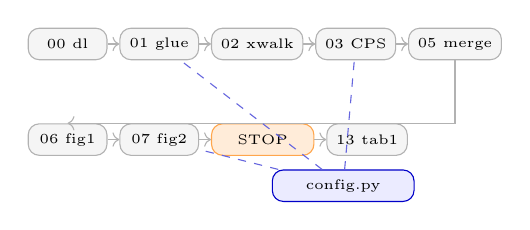
\begin{tikzpicture}[
    node distance=0.15cm,
    pstep/.style={rectangle, rounded corners, draw=gray!60, fill=gray!8,
        minimum width=1.0cm, minimum height=0.4cm, font=\tiny, text=DarkText, align=center},
    cfg/.style={rectangle, rounded corners, draw=RedTitle, fill=blue!8,
        minimum width=1.8cm, minimum height=0.4cm, font=\tiny, text=DarkText},
    gate/.style={rectangle, rounded corners, draw=orange!70, fill=orange!15,
        minimum width=1.3cm, minimum height=0.4cm, font=\tiny, text=DarkText, align=center}
]
\node[pstep] (s0) {00 dl};
\node[pstep, right=of s0] (s1) {01 glue};
\node[pstep, right=of s1] (s2) {02 xwalk};
\node[pstep, right=of s2] (s3) {03 CPS};
\node[pstep, right=of s3] (s5) {05 merge};
\node[pstep, below=0.8cm of s0] (s6) {06 fig1};
\node[pstep, right=of s6] (s7) {07 fig2};
\node[gate, right=of s7] (gate) {STOP};
\node[pstep, right=of gate] (s13) {13 tab1};
\node[cfg] (cfg) at (3.5, -1.8) {config.py};
\draw[->, gray!60] (s0) -- (s1);
\draw[->, gray!60] (s1) -- (s2);
\draw[->, gray!60] (s2) -- (s3);
\draw[->, gray!60] (s3) -- (s5);
\draw[->, gray!60] (s5.south) |- (s6.north);
\draw[->, gray!60] (s6) -- (s7);
\draw[->, gray!60] (s7) -- (gate);
\draw[->, gray!60] (gate) -- (s13);
\draw[dashed, RedTitle!60] (cfg) -- (s1);
\draw[dashed, RedTitle!60] (cfg) -- (s3);
\draw[dashed, RedTitle!60] (cfg) -- (s7);
\end{tikzpicture}
\end{center}
\end{column}
\begin{column}{0.46\textwidth}
\textbf{STOP GATE} before Table 1.
\begin{tcolorbox}[colback=gray!5,colframe=gray!40]
\begin{lstlisting}[style=pythonstyle,numbers=none,basicstyle=\ttfamily\scriptsize,language={}]
=== Figure 2 Inspection ===
 Group 3 (High AI, Low Glue):
   pre=94.6  post=89.0  d=-5.6
 Group 4 (High AI, High Glue):
   pre=99.5  post=99.8  d=+0.2
\end{lstlisting}
\end{tcolorbox}
\begin{itemize}\scriptsize
  \item Gate passes: Groups 3 and 4 diverge after Nov 2022; Table 1 is worth computing.
  \item Gate fails: inspect the proxy first. A regression table before the gate is false precision.
\end{itemize}
\end{column}
\end{columns}
\end{frame}

% ============================================================
% Frame 5.10 --- Act 4: Sign Reversal
% ============================================================
\begin{frame}{Act 4 --- When the Interaction Flips Sign}
On Apr 15 22:30 the earliest \texttt{glue\_core\_z} run produced an uncomfortable pattern:

\vspace{0.1cm}
\begin{tcolorbox}[colback=gray!5,colframe=gray!40]
\footnotesize
Glue content \textbf{reverses sign} depending on AI exposure:
\begin{itemize}\footnotesize
  \item Among low-AI occupations: High Glue $\to$ $+27$~pp better outcome than Low Glue.
  \item Among high-AI occupations: High Glue $\to$ $-15$~pp \emph{worse} outcome than Low Glue.
\end{itemize}
The interaction (AI $\times$ Glue) is negative. The simple ``glue protects bundles'' story predicts a positive interaction. --- \texttt{critical\_review\_and\_research\_directions.md}
\end{tcolorbox}

\vspace{0.15cm}
\begin{columns}[T]
\begin{column}{0.48\textwidth}
\textbf{Two readings}
\begin{itemize}\scriptsize
  \item (a) the theory is wrong;
  \item (b) the proxy conflates ``coordination present'' with ``coordination dominant'' and pools AI-easy documentation with AI-hard care.
\end{itemize}
\end{column}
\begin{column}{0.48\textwidth}
\textbf{Reframe chosen}
\begin{itemize}\scriptsize
  \item Protection operates through occupational \emph{reallocation}, not within-occupation survival.
  \item Coordination-secondary occupations (analysts) decline; coordination-primary ones (nurses) absorb the reallocation.
  \item The negative interaction is consistent with the theory once Condition 2 (sufficient coordination capacity) is stated explicitly.
\end{itemize}
\end{column}
\end{columns}
\end{frame}

% ============================================================
% Frame 5.11 --- Better Measures: the Four-Index Family
% ============================================================
\begin{frame}{Better Measures --- the Four-Index Family}
\scriptsize
\begin{tabular}{p{2.2cm}p{3.0cm}p{3.0cm}p{3.4cm}}
\toprule
\textbf{Index} & \textbf{What it captures} & \textbf{Construction} & \textbf{Why it matters} \\
\midrule
\texttt{glue\_core\_z} & baseline coordination bundle & 5-item coordination average & starting diagnostic, but contaminated \\
\texttt{glue\_aihard\_z} & embodied / relational coordination & keeps only human-hard items & drops LLM-easy pseudo-glue \\
\texttt{glue\_dominance\_z} & whether coordination is central & glue items relative to full activity bundle & separates primary from secondary coordination \\
\texttt{glue\_protection\_z} & replacement-risk composite & weighted mix of hard glue, dominance, social skill, AI-easy penalty & closest summary measure for the paper \\
\bottomrule
\end{tabular}

\vspace{0.18cm}
\begin{tcolorbox}[colback=blue!3,colframe=RedTitle!60]\scriptsize
\textbf{Pedagogical point.} Stage 1 did not stop at one index. It built a small family of measures so the economist could ask which pattern survives once the naive glue score is decomposed.
\end{tcolorbox}
\end{frame}

% ============================================================
% Frame 5.12 --- AI-hard vs AI-easy coordination
% ============================================================
\begin{frame}{Better Measures --- AI-Hard vs.\ AI-Easy Coordination}
\begin{columns}[T]
\begin{column}{0.48\textwidth}
\textbf{AI-hard coordination items}
\begin{itemize}\scriptsize
  \item Communicating with supervisors, peers, and subordinates
  \item Establishing and maintaining relationships
  \item Assisting and caring for others
  \item Coaching and developing others
  \item Resolving conflicts and negotiating
\end{itemize}
\end{column}
\begin{column}{0.48\textwidth}
\textbf{AI-easy pseudo-glue items}
\begin{itemize}\scriptsize
  \item Documenting and recording information
  \item Updating and using relevant knowledge
  \item Interpreting information for others
\end{itemize}
\vspace{0.1cm}
\scriptsize
The O*NET codes still live in the project config; the slide keeps the economic distinction rather than the implementation detail.
\end{column}
\end{columns}

\vspace{0.12cm}
\begin{tcolorbox}[colback=blue!3,colframe=RedTitle!60]\scriptsize
\textbf{Why split them?} A radiologist and a nurse may both coordinate, but only some coordination is hard for AI to absorb. That is the distinction the refined measures are trying to preserve.
\end{tcolorbox}
\end{frame}

% ============================================================
% Frame 5.13 --- Reading Figures
% ============================================================
\begin{frame}{Reading Figures, Suggesting Further Analysis}
\begin{columns}[T]
\begin{column}{0.5\textwidth}
\begin{center}

\includegraphics[height=0.6\textheight]{case5/fig_quadrants.png}
\end{center}
\end{column}
\begin{column}{0.46\textwidth}
\small\textbf{What this quadrant plot triggers.}
\begin{itemize}\scriptsize
  \item AI exposure and Glue Protection are only weakly correlated.
  \item The high-exposure column already splits into two populations.
  \item Bottom-right occupations look very different from top-right occupations.
  \item A single high-AI average would hide the mechanism.
\end{itemize}
\vspace{0.1cm}
\scriptsize
\textbf{Next move.} Compare high-protection and low-protection occupations \emph{within} the high-AI column. That request became the differential figure.
\end{column}
\end{columns}
\end{frame}

% ============================================================
% Frame 5.14 --- Headline figure
% ============================================================
\begin{frame}{The Headline Figure --- Four-Group Employment Trajectories}
\begin{center}

\includegraphics[height=0.66\textheight]{case5/fig_4group_trajectory.png}
\end{center}

\vspace{0.08cm}
\begin{tcolorbox}[colback=blue!3,colframe=RedTitle!60]\scriptsize
\textbf{Reading.} Once occupations are split by both AI exposure and Glue Protection, the trajectories are no longer pooled together. The theory claim is descriptive: similar AI exposure can coexist with different long-run employment paths.
\end{tcolorbox}
\end{frame}

% ============================================================
% Frame 5.15 --- Companion differential figure
% ============================================================
\begin{frame}{The Companion Figure --- Inside the High-AI Column}
\begin{center}

\includegraphics[height=0.68\textheight]{case5/fig_highai_differential.png}
\end{center}

\vspace{0.08cm}
\begin{tcolorbox}[colback=blue!3,colframe=RedTitle!60]\scriptsize
\textbf{Why this matters.} The ratio plot asks the cleaner question: among occupations with high AI exposure, do the high-protection occupations evolve differently from the low-protection occupations? That is the direct diagnostic behind the mechanism story.
\end{tcolorbox}
\end{frame}

% ============================================================
% Frame 5.16 --- Diagnostic Suite
% ============================================================
\begin{frame}{The Diagnostic Suite}
\scriptsize
\begin{tabular}{p{3.7cm}p{3.5cm}p{4.8cm}}
\toprule
\textbf{Diagnostic} & \textbf{What it asks} & \textbf{Where it lives (and what it found)} \\
\midrule
Management contamination & Is \texttt{glue\_core} just measuring whether the SOC prefix is ``11''? & Script 01 prints \texttt{corr(glue, is\_mgmt)} and warns when $>0.4$. \\
Sector residual (\texttt{glue\_sector\_z}) & Is glue just healthcare vs.\ production? & Partial out major-group means before re-ranking. \\
O*NET multi-wave (23.3 vs.\ 30.2) & Did task importance shift differentially in high-AI occupations? & Script 04: $\hat{\beta}_3 \approx 0$, $p\approx 0.52$. Attributed to the 2022--23 O*NET field lag. \\
Pre-trend decomposition (D1) & Is the divergence post-2022 or part of a long-run drift? & \texttt{figure\_pretrend\_allgroups\_longrun\_annual.png}: drift predates 2022. \\
\bottomrule
\end{tabular}

\vspace{0.2cm}
\begin{tcolorbox}[colback=blue!3,colframe=RedTitle!60]\scriptsize
\textbf{Rule.} Every claim in the snapshot is paired with the diagnostic that could have falsified it. The diagnostic lives on disk with a deterministic name.
\end{tcolorbox}
\end{frame}

% ============================================================
% Frame 5.15 --- Three-Document Writing Architecture
% ============================================================
\begin{frame}{Act 5 --- Three-Document Writing Architecture}
\begin{center}
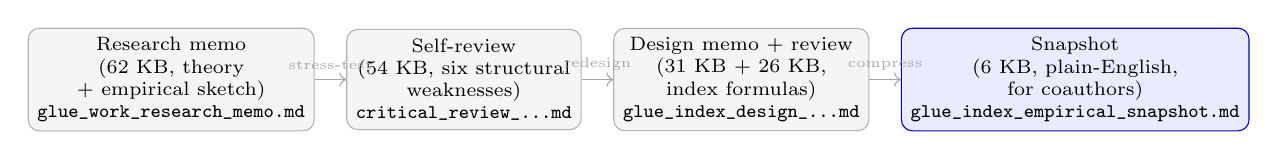
\begin{tikzpicture}[
    node distance=0.4cm,
    doc/.style={rectangle, rounded corners, draw=gray!60, fill=gray!8,
        minimum width=2.9cm, minimum height=1.05cm, font=\scriptsize, text=DarkText, align=center},
    snap/.style={rectangle, rounded corners, draw=RedTitle, fill=blue!8,
        minimum width=2.9cm, minimum height=1.05cm, font=\scriptsize, text=DarkText, align=center}
]
\node[doc] (memo) {Research memo\\(62~KB, theory\\+ empirical sketch)\\\scriptsize\texttt{glue\_work\_research\_memo.md}};
\node[doc, right=of memo] (review) {Self-review\\(54~KB, six structural\\weaknesses)\\\scriptsize\texttt{critical\_review\_...md}};
\node[doc, right=of review] (design) {Design memo + review\\(31~KB + 26~KB,\\index formulas)\\\scriptsize\texttt{glue\_index\_design\_...md}};
\node[snap, right=of design] (snapshot) {Snapshot\\(6~KB, plain-English,\\for coauthors)\\\scriptsize\texttt{glue\_index\_empirical\_snapshot.md}};
\draw[->, gray!70] (memo) -- node[above, font=\tiny]{stress-test} (review);
\draw[->, gray!70] (review) -- node[above, font=\tiny]{redesign} (design);
\draw[->, gray!70] (design) -- node[above, font=\tiny]{compress} (snapshot);
\end{tikzpicture}
\end{center}

\vspace{0.15cm}
\textbf{Each step has one job.} The memo names the claim. The self-review tries to break it. The design memos rebuild the measure so the claim survives scrutiny. The snapshot delivers the survivor to a coauthor in one page. Writing one document for all four purposes produces a paper that defends everything badly.
\end{frame}

% ============================================================
% Frame 5.16 --- From Memo to Snapshot
% ============================================================
\begin{frame}{Refining --- From Memo to Snapshot}
\begin{columns}[T]
\begin{column}{0.48\textwidth}
\textbf{Memo opener} (argumentative, for the reviewer)
\begin{tcolorbox}[colback=gray!5,colframe=gray!40]
\scriptsize
A central question in the economics of AI is whether and how artificial intelligence displaces workers. Garicano, Li, and Wu (2026) push back \dots by arguing that labor markets price \emph{jobs}, not isolated tasks. \dots This memo argues that \textbf{glue work} is the missing microfoundation for bundle strength.
\end{tcolorbox}
\end{column}
\begin{column}{0.48\textwidth}
\textbf{Snapshot bottom line} (declarative, for the coauthor)
\begin{tcolorbox}[colback=gray!5,colframe=gray!40]
\scriptsize
Two occupations can have the same AI exposure and different labor-market trajectories. The Glue Protection index is an attempt to name one dimension along which they differ. The construction is declarative and inspectable; the next question is how to rationalize the pattern.
\end{tcolorbox}
\end{column}
\end{columns}

\vspace{0.2cm}
\begin{itemize}\scriptsize
  \item Compression ratio: $\sim 62$~KB memo $\to$ $\sim 6$~KB snapshot, roughly $10\times$.
  \item Audience shift: reviewer (argue for the framework) $\to$ coauthor (inspect the data).
  \item Vocabulary shift: ``microfoundation'' $\to$ ``two occupations''; theoretical verbs $\to$ empirical verbs.
\end{itemize}
\end{frame}

% ============================================================
% Frame 5.17 --- Spotting Issues, Open Threads
% ============================================================
\begin{frame}{Spotting Issues, Naming Open Threads}
\scriptsize
\begin{tabular}{p{3.7cm}p{3.3cm}p{5.0cm}}
\toprule
\textbf{Issue} & \textbf{Where surfaced} & \textbf{Disposition} \\
\midrule
Bartik shock infeasible & Act 2 data scan (BTOS Q7 suppressed at sector) & deferred; wait for a richer AI-adoption panel \\
\texttt{glue\_core} contaminated by LLM-easy items & Apr 15 self-review & \texttt{glue\_aihard\_z} promoted to co-primary; \texttt{glue\_aieasy\_z} added as penalty \\
Coordination-presence vs.\ dominance & Apr 17 review & \texttt{glue\_dominance\_z} added (mean glue $\div$ mean 41 activities) \\
Webb (2020) not integrated & crosswalk triage (occ1990dd $\to$ Census 2018 not built) & parked as robustness; waits on a new crosswalk \\
O*NET multi-wave null ($\hat\beta_3\approx 0$) & Script 04 diagnostic & attributed to 2022--23 field lag; rerun on O*NET 31 when released \\
\bottomrule
\end{tabular}

\vspace{0.2cm}
\begin{tcolorbox}[colback=blue!3,colframe=RedTitle!60]\scriptsize
Each row is where the next sprint starts. A sprint that ends without a written issue list starts the next sprint by rediscovering its own unsolved problems.
\end{tcolorbox}
\end{frame}

% ============================================================
% Frame 5.18 --- Division of Labor Move by Move
% ============================================================
\begin{frame}{Division of Labor --- Move by Move}
\scriptsize
\begin{tabular}{p{3.1cm}p{4.2cm}p{4.7cm}}
\toprule
\textbf{Move} & \textbf{Agent did} & \textbf{Economist did} \\
\midrule
Name the puzzle & draft the three-sentence opener from a literature sweep & chose GLW (2026) as the anchor; named glue work as the missing microfoundation \\
Choose O*NET items & proposed five items from the content model & vetoed three LLM-easy items; added the embodied/relational list \\
Build the pipeline & wrote scripts 00--14, wired \texttt{config.py}, added 51 unit tests & locked the parameter values and the STOP GATE criterion \\
Spot sign reversal & printed the pre/post deltas; surfaced the pattern & recognised it as a theory problem, not a bug \\
Reframe theory & produced three candidate rewordings & chose reallocation-not-survival; wrote the new abstract \\
Design the four-index family & drafted \texttt{aihard}, \texttt{dominance}, \texttt{social}, \texttt{aieasy} with weights & fixed the 35/25/25/15 weights; named the composite \\
Write the snapshot & compressed 62~KB $\to$ 6~KB on request & read the draft as a coauthor would; rewrote the bottom line \\
\bottomrule
\end{tabular}

\vspace{0.2cm}
\textbf{The constant.} The agent executes; the economist decides what is true. The economist's work is not replaced --- it is concentrated into judgment calls.
\end{frame}

% ============================================================
% Frame 5.19 --- End of Stage 1: Memo + Coauthor Discussion
% ============================================================
\begin{frame}{End of Stage 1 --- Memo, Critique, and What Triggered Stage 2}
\begin{columns}[T]
\begin{column}{0.32\textwidth}
\textbf{The memo (6 KB)}
\begin{tcolorbox}[colback=gray!5,colframe=gray!40]\scriptsize
\emph{``Two occupations can have the same AI exposure and different labor-market trajectories. Glue Protection names one possible reason. The construction is inspectable; the next step is to explain the pattern.''}
\end{tcolorbox}
\scriptsize One page, plain English, readable by a coauthor in three minutes.
\end{column}
\begin{column}{0.32\textwidth}
\textbf{The coauthor critique}
\begin{tcolorbox}[colback=gray!5,colframe=RedTitle!60]\scriptsize
\textbf{Apr~18 critique:}
\begin{itemize}\scriptsize
  \item ``You're still using the mean of a within-occupation distribution. The \emph{shape} matters.''
  \item ``If two tasks have very different exposures, the job gets \emph{unbundled} --- not \emph{substituted}.''
  \item ``Add a second measure: how dispersed is the exposure \emph{within} an occupation?''
\end{itemize}
\end{tcolorbox}
\end{column}
\begin{column}{0.32\textwidth}
\textbf{The question that launched Stage 2}
\begin{tcolorbox}[colback=blue!3,colframe=RedTitle!60]\small
\emph{Holding mean AI exposure fixed, does within-job dispersion of exposure predict labor-share outcomes?}
\end{tcolorbox}

\vspace{0.12cm}\scriptsize
That question became the Stage 2 workflow over the next week.
\end{column}
\end{columns}

\vspace{0.12cm}
\begin{tcolorbox}[colback=blue!3,colframe=RedTitle!60]\scriptsize
\textbf{Rule.} A short memo plus an honest critique is the cheapest way to make the next sprint smarter.
\end{tcolorbox}
\end{frame}

%===========================================================
\sectiondivider{Case Study 5 --- Stages 2, 3, 4}{From a single glue index to a distribution --- and an LLM-built index in between}
%===========================================================

% ============================================================
% Frame 5.20 --- Stage 2 opens
% ============================================================
\begin{frame}{Stage 2 --- AI Task Dispersion (opens)}
\begin{columns}[T]
\begin{column}{0.5\textwidth}
\textbf{Question.} Given the mean AI exposure $\bar E_o$, does within-occupation dispersion of exposure predict labor-share movement?

\vspace{0.1cm}
\textbf{Data (new).} Add \textbf{Eloundou et~al.~(2023)} GPT-4 $T$-scores as a second, independent AI-exposure source parallel to FRS. Tasks, not abilities. 13{,}225 Core tasks across 872 O*NET-SOC codes.

\vspace{0.1cm}
\textbf{Strategy.} Per-occupation features (\texttt{task\_count}, \texttt{ai\_exposure\_sd}) built at O*NET-SOC, bridged through SOC~2018 $\to$ OCC1950 via CPS-weighted pairs. Outcome: $\Delta$share in an OCC1950 $\times$ (age $\times$ education) cell.
\end{column}
\begin{column}{0.48\textwidth}
\textbf{Report.} Coefficient tables for Experiments A--E across four cells and two sources. Binscatter figures.

\vspace{0.1cm}
\textbf{Analyze.} Nested WLS ladder weighted by pre-period employment share, HC1 SEs:
\begin{itemize}\scriptsize
  \item M0: $\Delta s \sim \bar E$
  \item M1: $\Delta s \sim \bar E + \text{SD}$
  \item M2: $\Delta s \sim \bar E + \text{TC}$
  \item M3: $\Delta s \sim \bar E + \text{SD} + \text{TC}$
\end{itemize}

\vspace{0.1cm}
\textbf{Interpret.} Does $|\hat\beta_{\text{SD}}|$ or $|\hat\beta_{\text{TC}}|$ rival $|\hat\beta_{\bar E}|$ on a 1-SD scale?
\end{column}
\end{columns}

\vspace{0.15cm}
\begin{tcolorbox}[colback=blue!3,colframe=RedTitle!60]\scriptsize
Same six-element template as Stage 1; different question. Pipeline home: \texttt{docs/ai\_task\_dispersion/ai\_task\_dispersion\_memo.tex}, Scripts \texttt{18, 18b, 19, 20, 21}.
\end{tcolorbox}
\end{frame}

% ============================================================
% Frame 5.21 --- Stage 2 Features and Specs
% ============================================================
\begin{frame}{Stage 2 --- Features, Specs, and the Head-to-Head Question}
\begin{columns}[T]
\begin{column}{0.48\textwidth}
\scriptsize
\textbf{Feature pairs per source}
\begin{tabular}{p{2.1cm}p{3.5cm}}
\toprule
\textbf{Source} & \textbf{Features} \\
\midrule
FRS (abilities) & \texttt{task\_count}, \texttt{ai\_exposure\_sd} — 52 abilities screened at IM $\ge 3$ \\
Eloundou (tasks) & \texttt{task\_count\_el}, \texttt{ai\_exposure\_sd\_el} — Core tasks, T-score 0--4 \\
\bottomrule
\end{tabular}

\vspace{0.2cm}
\textbf{The head-to-head.} All features z-scored within cell so the ratio $|\hat\beta_{\text{feat}}/\hat\beta_{\bar E}|$ says ``how many 1-SD of $\bar E$ does a 1-SD of the feature deliver?''
\end{column}
\begin{column}{0.48\textwidth}
\begin{center}

\includegraphics[height=0.58\textheight]{case5/shapley_stacked.png}
\end{center}
\vspace{-0.2cm}
{\scriptsize \textbf{Experiment E Shapley decomposition (FRS side).} Each cell's full-model $R^2$ split across $\{\bar E,\ \text{SD},\ \text{TC}\}$ by average marginal contribution across orderings.}
\end{column}
\end{columns}
\end{frame}

% ============================================================
% Frame 5.22 --- Stage 2 Findings
% ============================================================
\begin{frame}{Stage 2 --- Three Findings}
\begin{enumerate}\small
  \item \textbf{Task count is robust.} Young~$\times$~College: $\hat\beta_{\text{TC}}=+0.0059$ ($p=0.005$) on FRS, $+0.0045$ ($p=0.002$) on Eloundou. Same sign, both sources, same cell. Carries 62--83\% of $R^2$ in the Shapley decomposition for that cell.
  \item \textbf{AI SD is cell-specific.} Significant under Eloundou in Young~$\times$~College ($p=0.018$ in M3) and under FRS in Middle~$\times$~Non-college ($p=0.005$). Elsewhere indistinguishable from zero. Not universal.
  \item \textbf{Mean AI exposure is \emph{not} a sufficient statistic.} In 5 of 8 cells the Shapley share of the mean-AI channel is below half. The residual share is concentrated in TC or SD depending on the cell.
\end{enumerate}

\vspace{0.2cm}
\begin{tcolorbox}[colback=gray!5,colframe=gray!40]\scriptsize
\textbf{Middle $\times$ Non-college (FRS; 36.7\% of prime-age employment).} $\hat\beta_{\bar E} = -0.0040$ (M1), $\hat\beta_{\text{SD}} = -0.0041$ (M1). Ratio $|\hat\beta_{\text{SD}}/\hat\beta_{\bar E}| \approx 1.01$, and SD adds $+15.8$pp to $R^2$ on top of mean AI alone. In this cell, within-job dispersion matches the mean-AI channel dollar-for-dollar.
\end{tcolorbox}
\end{frame}

% ============================================================
% Frame 5.23 --- End of Stage 2
% ============================================================
\begin{frame}{End of Stage 2 --- Memo, Critique, What Launched Stage 3}
\begin{columns}[T]
\begin{column}{0.32\textwidth}
\textbf{The memo}
\begin{tcolorbox}[colback=gray!5,colframe=gray!40]\scriptsize
\texttt{ai\_task\_dispersion\_memo.tex} --- 14 pages, five experiments, descriptive throughout.

\vspace{0.1cm}
Bottom line: the task-count finding survives replication; within-job SD is a second channel with cell-specific bite; mean AI exposure is not a sufficient statistic.
\end{tcolorbox}
\end{column}
\begin{column}{0.32\textwidth}
\textbf{The coauthor critique}
\begin{tcolorbox}[colback=gray!5,colframe=RedTitle!60]\scriptsize
\begin{itemize}\scriptsize
  \item ``Task count tells you the \emph{number} of tasks. But not whether each task is AI-\emph{substitute} or AI-\emph{assist}.''
  \item ``Eloundou gives one $T$-score per task. You need \emph{two}: $e_{\text{sub}}$ and $e_{\text{asst}}$.''
  \item ``Can the LLM itself do this for 13{,}000 tasks?''
\end{itemize}
\end{tcolorbox}
\end{column}
\begin{column}{0.32\textwidth}
\textbf{What launches Stage 3}
\begin{tcolorbox}[colback=blue!3,colframe=RedTitle!60]\small
\emph{Build a task-level LLM-labeled index that decomposes AI exposure into substitution and assistance.}
\end{tcolorbox}
\vspace{0.15cm}\scriptsize
This seeds Scripts 22--29 and the \texttt{unbundling\_vulnerability} track.
\end{column}
\end{columns}
\end{frame}

% ============================================================
% Frame 5.24 --- Stage 3 opens
% ============================================================
\begin{frame}{Stage 3 --- Unbundling Vulnerability (opens)}
\begin{columns}[T]
\begin{column}{0.48\textwidth}
\textbf{The missing decomposition.}

Both FRS AIOE and Eloundou $T$-score deliver \emph{one} number per task or ability. That number bundles two qualitatively different things:
\begin{itemize}\small
  \item $e_{\text{sub}}$ --- AI can \emph{replace} the worker on this task;
  \item $e_{\text{asst}}$ --- AI can \emph{help} the worker do this task faster.
\end{itemize}

\vspace{0.1cm}
A scholar with one task at $e=0.8$ and a call-center agent with one task at $e=0.8$ have the same AIOE score --- and likely very different labor-market trajectories.
\end{column}
\begin{column}{0.48\textwidth}
\textbf{What the LLM can do that the literature can't.}

The O*NET task description plus a rubric is enough for a modern LLM to distinguish the two readings task-by-task. 13{,}225 tasks $\times$ (sub, asst) scores is $\sim$26{,}000 new data points that do not exist in any public release.

\vspace{0.15cm}
\textbf{Deliverables.}
\begin{itemize}\small
  \item $R_o = E_{\text{sub}}/(E_{\text{sub}}+E_{\text{asst}}+\epsilon)$ --- occupation-level substitution share.
  \item $U_o$ --- composite Unbundling Vulnerability Index that uses $R_o$.
\end{itemize}
\end{column}
\end{columns}

\vspace{0.2cm}
\begin{tcolorbox}[colback=blue!3,colframe=RedTitle!60]\scriptsize
\textbf{The LLM can score something the original index was never built to see.} Home: \texttt{docs/unbundling\_vulnerability/}.
\end{tcolorbox}
\end{frame}

% ============================================================
% Frame 5.25 --- The Ambition
% ============================================================
\begin{frame}{Stage 3 --- The Ambition: Scoring 13{,}225 Tasks}
\begin{columns}[T]
\begin{column}{0.5\textwidth}
\scriptsize
\begin{tabular}{lr}
\toprule
Corpus size & \textbf{13{,}225} O*NET Core tasks \\
Per-task output & $(e_{\text{sub}}, e_{\text{asst}}, \text{rationale})$ in $[0,1]$ \\
Calls required (na\"ive) & 13{,}225 LLM calls \\
Budget at Claude Max & one 5-hour window \\
Strategy & \textbf{bulk + adjudicate + cache} \\
\bottomrule
\end{tabular}

\vspace{0.25cm}
\textbf{Three design moves} that turn a 13k-call ambition into a tractable pipeline:
\begin{itemize}\scriptsize
  \item \textbf{Bulk}: 10 tasks per Haiku call --- one JSON array in, one JSON array out. Cuts calls by 10$\times$.
  \item \textbf{Adjudicate}: Sonnet reruns the tasks Haiku flagged as borderline.
  \item \textbf{Cache}: one file per task on disk; re-runs skip already-labeled tasks. Interruption-proof.
\end{itemize}
\end{column}
\begin{column}{0.48\textwidth}
\textbf{Why each move matters}
\begin{tcolorbox}[colback=gray!5,colframe=gray!40]\scriptsize
Without bulking: 13k calls $\times \sim 10$s $= \sim$36~hours --- no single Claude Max window fits.

\vspace{0.1cm}
Without adjudication: Haiku's borderline judgments carry the whole index; no second opinion, no way to flag hard cases.

\vspace{0.1cm}
Without caching: any network blip, quota limit, or power loss destroys hours of work. The 5-hour window \emph{will} expire mid-run --- the cache turns that from a catastrophe into a coffee break.
\end{tcolorbox}
\vspace{0.1cm}
\textbf{Script home.} \texttt{scripts/24\_label\_substitution\_assistance.py}.
\end{column}
\end{columns}
\end{frame}

% ============================================================
% Frame 5.26 --- The Architecture (TikZ flow)
% ============================================================
\begin{frame}{Stage 3 --- The Labeling Architecture}
\begin{center}
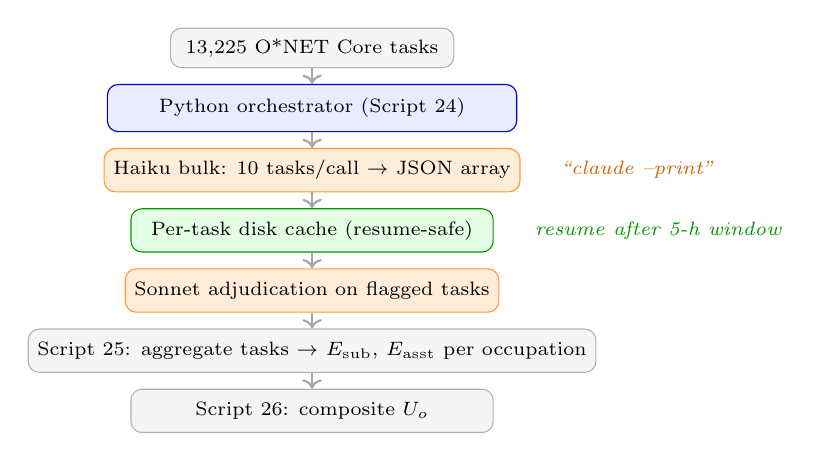
\begin{tikzpicture}[
    node distance=0.2cm,
    src/.style={rectangle, rounded corners, draw=gray!60, fill=gray!8,
        minimum width=3.6cm, minimum height=0.5cm, font=\scriptsize, text=DarkText, align=center},
    orch/.style={rectangle, rounded corners, draw=RedTitle, fill=blue!8,
        minimum width=5.2cm, minimum height=0.6cm, font=\scriptsize, text=DarkText, align=center},
    llm/.style={rectangle, rounded corners, draw=orange!80, fill=orange!15,
        minimum width=4.6cm, minimum height=0.55cm, font=\scriptsize, text=DarkText, align=center},
    cache/.style={rectangle, rounded corners, draw=green!60!black, fill=green!10,
        minimum width=4.6cm, minimum height=0.55cm, font=\scriptsize, text=DarkText, align=center},
    agg/.style={rectangle, rounded corners, draw=gray!60, fill=gray!8,
        minimum width=4.6cm, minimum height=0.55cm, font=\scriptsize, text=DarkText, align=center},
    flow/.style={->, gray!70, thick}
]
\node[src] (tasks) {13{,}225 O*NET Core tasks};
\node[orch, below=of tasks] (orch) {Python orchestrator (Script 24)};
\node[llm, below=of orch] (haiku) {Haiku bulk: 10 tasks/call $\to$ JSON array};
\node[cache, below=of haiku] (cache) {Per-task disk cache (resume-safe)};
\node[llm, below=of cache] (sonnet) {Sonnet adjudication on flagged tasks};
\node[agg, below=of sonnet] (agg1) {Script 25: aggregate tasks $\to$ $E_{\text{sub}},\,E_{\text{asst}}$ per occupation};
\node[agg, below=of agg1] (agg2) {Script 26: composite $U_o$};

\draw[flow] (tasks) -- (orch);
\draw[flow] (orch) -- (haiku);
\draw[flow] (haiku) -- (cache);
\draw[flow] (cache) -- (sonnet);
\draw[flow] (sonnet) -- (agg1);
\draw[flow] (agg1) -- (agg2);

\node[right=0.4cm of cache, text=green!60!black, font=\scriptsize\itshape] {resume after 5-h window};
\node[right=0.4cm of haiku, text=orange!80!black, font=\scriptsize\itshape] {``claude --print''};
\end{tikzpicture}
\end{center}

\vspace{-0.05cm}
\begin{tcolorbox}[colback=blue!3,colframe=RedTitle!60]\scriptsize
\textbf{Three layers of LLM.} Claude Code writes Python (layer 1); the Python spawns \texttt{claude --print} Haiku sessions (layer 2); Sonnet adjudicates the borderline cases (layer 3). \textbf{11{,}171 of 13{,}225 tasks labeled (84.5\%)} in one 5-hour window before the quota expired. Resume via cache; no task re-labeled.
\end{tcolorbox}
\end{frame}

% ============================================================
% Frame 5.27 --- The Prompt
% ============================================================
\begin{frame}{Stage 3 --- The Rubric Behind the Labels}
\begin{columns}[T]
\begin{column}{0.48\textwidth}
\textbf{Replacement score $e_{\text{sub}}$}
\begin{itemize}\scriptsize
  \item 0.00: AI cannot replace the task
  \item 0.25: AI handles only narrow pieces
  \item 0.50: human and AI split the task
  \item 0.75: AI does most of the work; human reviews
  \item 1.00: AI replaces the task almost entirely
\end{itemize}
\end{column}
\begin{column}{0.48\textwidth}
\textbf{Assistive score $e_{\text{asst}}$}
\begin{itemize}\scriptsize
  \item 0.00: no productivity gain
  \item 0.25: speeds up a narrow sub-step
  \item 0.50: roughly doubles throughput
  \item 0.75: handles most of the time cost
  \item 1.00: task becomes trivial once AI is used
\end{itemize}
\end{column}
\end{columns}

\vspace{0.12cm}
\begin{tcolorbox}[colback=gray!5,colframe=gray!40]\scriptsize
\textbf{Three anchors.} Clear substitute: \emph{transcribe audio}. Clear assistant: \emph{perform laparoscopic surgery}. Borderline case: \emph{draft a legal contract clause}. Input was a batch of 10 tasks; output was structured JSON with scores, rationale, and an ambiguity flag.
\end{tcolorbox}
\end{frame}

% ============================================================
% Frame 5.28 --- Token engineering detail
% ============================================================
\begin{frame}{Stage 3 --- Token Engineering at Scale}
\begin{columns}[T]
\begin{column}{0.48\textwidth}
\textbf{Operational trick}
\begin{tcolorbox}[colback=gray!5,colframe=gray!40]\scriptsize
Run \texttt{claude --print} from a clean temporary directory so the project's 12k-token \texttt{CLAUDE.md} does \emph{not} auto-load into every bulk call.
\end{tcolorbox}

\vspace{0.12cm}
\textbf{Why it matters}
\begin{itemize}\scriptsize
  \item 13k tasks means thousands of repeated API calls.
  \item Small prompt waste becomes massive token waste.
  \item Cheap calls stay cheap only if the context stays minimal.
\end{itemize}
\end{column}
\begin{column}{0.48\textwidth}
\textbf{Economic interpretation}
\begin{tcolorbox}[colback=blue!3,colframe=RedTitle!60]\scriptsize
\textbf{Saved scale.} About 160M tokens avoided over the full run. At this scale, prompt engineering is not cosmetic; it is cost control and latency control.
\end{tcolorbox}

\vspace{0.12cm}
\textbf{Teaching point}
\begin{itemize}\scriptsize
  \item The rubric stayed constant.
  \item The execution environment changed.
  \item Agentic AI is strongest when the human specifies the rule once and the system executes it thousands of times.
\end{itemize}
\end{column}
\end{columns}
\end{frame}

% ============================================================
% Frame 5.29 --- Running Massive Work Unsupervised
% ============================================================
\begin{frame}[fragile]{Stage 3 --- Running Massive Work Unsupervised}
\begin{columns}[T]
\begin{column}{0.48\textwidth}
\textbf{What the economist did.}
\begin{itemize}\scriptsize
  \item Wrote the rubric (\textasciitilde{}30 lines) and three calibration anchors.
  \item Read $\sim$12 LLM-returned labels by eye to sanity-check the scale.
  \item Launched the run and walked away.
\end{itemize}

\vspace{0.15cm}
\textbf{What Claude Code did.}
\begin{itemize}\scriptsize
  \item Wrote the orchestrator (Script 24).
  \item Spawned thousands of \texttt{claude --print} Haiku sessions.
  \item Wrote each task's result to its own cache file.
  \item Detected quota expiration, logged cleanly, exited gracefully.
\end{itemize}

\vspace{0.15cm}
\textbf{What the LLM (Haiku/Sonnet) did.}
\begin{itemize}\scriptsize
  \item Returned $(e_{\text{sub}}, e_{\text{asst}})$ for 11{,}171 tasks on the first pass.
  \item Flagged 3{,}456 ambiguous tasks for adjudication.
\end{itemize}
\end{column}
\begin{column}{0.48\textwidth}
\textbf{Log excerpt} (\texttt{script24\_bulk\_run.log}):
\begin{tcolorbox}[colback=gray!5,colframe=gray!40]
\begin{lstlisting}[style=pythonstyle,numbers=none,basicstyle=\ttfamily\tiny,language={}]
06:41:22 INFO  batch 1108 (10 tasks) -> 10 cached
06:41:41 INFO  batch 1109 (10 tasks) -> 10 cached
06:42:01 INFO  batch 1110 (10 tasks) -> 10 cached
...
11:28:03 INFO  rate-limit backoff (45s)
11:28:48 INFO  batch 1117 (10 tasks) -> 10 cached
11:29:57 ERROR claude-max window expired
11:29:57 INFO  cache now holds 11,171/13,225 tasks
11:29:57 INFO  resume via: python scripts/24_...py --skip-gates
\end{lstlisting}
\end{tcolorbox}

\vspace{0.1cm}
\begin{tcolorbox}[colback=blue!3,colframe=RedTitle!60]\scriptsize
\textbf{Supervision cost.} $\sim 20$ minutes of economist time to spec the rubric. $\sim 5$ hours of unsupervised LLM work. $\sim 12$ labels read by eye out of 11{,}171. This is the ratio that makes LLM labeling a viable empirical tool at corpus scale.
\end{tcolorbox}
\end{column}
\end{columns}
\end{frame}

% ============================================================
% Frame 5.30 --- From Tasks to U_o
% ============================================================
\begin{frame}{Stage 3 --- From per-Task Scores to $U_o$}
\textbf{Task $\to$ occupation aggregation} (Script 25):
\[
E^{\text{sub}}_o = \sum_t w_t \cdot e^{\text{sub}}_t, \quad
E^{\text{asst}}_o = \sum_t w_t \cdot e^{\text{asst}}_t
\]
\[
R_o = \frac{E^{\text{sub}}_o}{E^{\text{sub}}_o + E^{\text{asst}}_o + \epsilon}
\]

\vspace{0.12cm}
\textbf{Composite} (Script 26):
\[
U_o = \alpha\,\bar E_o + \beta\,V_o + \theta\,T_o + \lambda\,(R_o \cdot \bar E_o) - \gamma\,C_o - \mu\,Q_o
\]

\vspace{0.08cm}
\begin{tcolorbox}[colback=gray!5,colframe=gray!40]\scriptsize
\textbf{Interpretation.} $V$ is within-job dispersion, $T$ is top-tail exposure, $C$ is coordination cost, and $Q$ is accountability intensity. The point is not that one scalar is perfect; it is that the index records several reasons a job may be vulnerable or protected.
\end{tcolorbox}
\end{frame}

% ============================================================
% Frame 5.31 --- Weight sensitivity
% ============================================================
\begin{frame}[fragile]{Stage 3 --- Weight Sensitivity of $U_o$}
\begin{columns}[T]
\begin{column}{0.42\textwidth}
\textbf{Declared weights} (\texttt{config.py:AUI\_WEIGHTS}, not data-fit):
\begin{tcolorbox}[colback=gray!5,colframe=gray!40]
\begin{lstlisting}[style=pythonstyle,numbers=none,basicstyle=\ttfamily\tiny,language={}]
AUI_WEIGHTS = {
    "E_bar":     0.30,
    "V":         0.15,
    "T":         0.20,
    "R_times_E": 0.15,
    "C_neg":     0.15,
    "Q_neg":     0.05,
}
\end{lstlisting}
\end{tcolorbox}
\end{column}
\begin{column}{0.54\textwidth}
\begin{center}

\includegraphics[height=0.52\textheight]{case5/aui_weight_sensitivity.png}
\end{center}
\end{column}
\end{columns}

\vspace{0.08cm}
\begin{tcolorbox}[colback=blue!3,colframe=RedTitle!60]\scriptsize
\textbf{Stability check.} The top and bottom occupations in $U_o$ survive reasonable re-weighting. That does not prove the weights are correct; it shows the ranking is not driven by one arbitrary coefficient choice.
\end{tcolorbox}
\end{frame}

% ============================================================
% Frame 5.32 --- Reading U_o
% ============================================================
\begin{frame}{Stage 3 --- Reading the $U_o$ Index}
\begin{center}

\includegraphics[height=0.60\textheight]{case5/aui_quadrants.png}
\end{center}

\vspace{0.04cm}
\begin{tcolorbox}[colback=blue!3,colframe=RedTitle!60]\scriptsize
\textbf{Quadrants.} Top-right occupations are wholesale-substitution candidates. Top-left occupations face reskilling pressure even when mean exposure is not especially high. The decomposition changes the stories at the margin, not only at the extremes.
\end{tcolorbox}
\end{frame}

% ============================================================
% Frame 5.33 --- Movers under U_o
% ============================================================
\begin{frame}{Stage 3 --- Where $U_o$ Changes the Ranking}
\begin{center}

\includegraphics[height=0.68\textheight]{case5/notable_movers.png}
\end{center}

\vspace{0.08cm}
\begin{tcolorbox}[colback=blue!3,colframe=RedTitle!60]\scriptsize
\textbf{Disagreement region.} The interesting cases are where $U_o$ and $P^{\text{rich}}$ disagree. That is exactly where the task-level labeling work pays off: it adds information the Stage 1 protection index could not recover.
\end{tcolorbox}
\end{frame}

% ============================================================
% Frame 5.34 --- End of Stage 3
% ============================================================
\begin{frame}{End of Stage 3 --- Memo, Critique, and Cost}
\begin{columns}[T]
\begin{column}{0.32\textwidth}
\textbf{The memo (partial)}
\begin{tcolorbox}[colback=gray!5,colframe=gray!40]\scriptsize
\texttt{unbundling\_vulnerability\_empirical\_snapshot.md} is populated \emph{partially} because Stage 3 paused with 2{,}054 remainder + 3{,}456 adjudication queued.

\vspace{0.1cm}
The design memo + LLM prompts + quadrant figures are complete; $R_o$ numbers are placeholder pending the remaining labels.
\end{tcolorbox}
\end{column}
\begin{column}{0.32\textwidth}
\textbf{The coauthor critique}
\begin{tcolorbox}[colback=gray!5,colframe=RedTitle!60]\scriptsize
Apr~22 call, Xiaojie Liu:

\vspace{0.1cm}
\emph{``Your top-tail share is 0.97 correlated with mean exposure. You still do not have an independent axis. The within-job \emph{shape of the distribution}, not the upper tail, is where you can learn something $\bar E$ does not carry.''}
\end{tcolorbox}
\end{column}
\begin{column}{0.32\textwidth}
\textbf{What launches Stage 4}
\begin{tcolorbox}[colback=blue!3,colframe=RedTitle!60]\small
\emph{Refine within-job distribution features; test each one against mean AI exposure.}
\end{tcolorbox}

\vspace{0.15cm}
\textbf{Cost accounting.}
\begin{tcolorbox}[colback=gray!5,colframe=gray!40]\scriptsize
$\sim$11k tasks $\times \sim$2 Haiku calls $\times \sim$300 tokens $\approx$ 7M tokens in one 5-h window. Cache guarantees no re-runs.
\end{tcolorbox}
\end{column}
\end{columns}
\end{frame}

% ============================================================
% Frame 5.32 --- Stage 4 opens
% ============================================================
\begin{frame}{Stage 4 --- Exposure Structure Refinement (opens)}
\begin{columns}[T]
\begin{column}{0.48\textwidth}
\textbf{Question.} Holding mean AI exposure $\bar E$ fixed, which \emph{distribution-shape} statistics of within-job exposure add information for labor-share outcomes?

\vspace{0.1cm}
\textbf{Data (no new source).} Same FRS + Eloundou inputs. What changes is the feature set: instead of just mean and SD, compute a family of shape statistics.

\vspace{0.1cm}
\textbf{Strategy.}
\begin{itemize}\scriptsize
  \item Tighten tail thresholds: p33 $\to$ p10 (FRS), $T\ge 3 \to T=4$ (Eloundou).
  \item Add \texttt{top\_bottom\_gap}, \texttt{top\_within\_mean}, \texttt{bottom\_quantile\_mean}, \texttt{importance\_rank\_slope}.
  \item Regress $\Delta$share on each feature (conditioning on $\bar E$), pooled and per-cell.
\end{itemize}
\end{column}
\begin{column}{0.48\textwidth}
\textbf{Report.}
\begin{itemize}\scriptsize
  \item Correlation-with-$\bar E$ table for every feature.
  \item F1 pairwise $\Delta R^2$ rankings.
  \item F5 focused horse race: $\beta(X) / \beta(\bar E)$ ratios.
  \item Shapley-on-4 allocating the increment over the $\bar E$-only baseline.
\end{itemize}

\vspace{0.1cm}
\textbf{Analyze.} Cluster-robust SEs at \texttt{occ1950} for pooled specs (each occupation contributes four cell-rows; HC1 understates). Script \texttt{21b\_run\_exposure\_structure\_regressions.py}.

\vspace{0.1cm}
\textbf{Interpret.} Which refined features beat $\bar E$ in magnitude? Which disappear once $\bar E$ is controlled?
\end{column}
\end{columns}
\end{frame}

% ============================================================
% Frame 5.36 --- Three Archetypes
% ============================================================
\begin{frame}{Stage 4 --- Three Archetypes of Within-Job Exposure}
\begin{center}

\includegraphics[height=0.64\textheight]{case5/archetypes_stylized.png}
\end{center}

\vspace{0.08cm}
\begin{tcolorbox}[colback=blue!3,colframe=RedTitle!60]\scriptsize
\textbf{Conceptual point.} Flat-low, flat-high, and bimodal jobs can share the same mean exposure while implying three different labor-market predictions: untouched, wholesale substitution, and unbundling.
\end{tcolorbox}
\end{frame}

% ============================================================
% Frame 5.37 --- Real analogues
% ============================================================
\begin{frame}{Stage 4 --- Real Analogues for the Three Archetypes}
\begin{center}

\includegraphics[height=0.60\textheight]{case5/archetypes_exemplar.png}
\end{center}

\vspace{0.08cm}
\begin{tcolorbox}[colback=blue!3,colframe=RedTitle!60]\scriptsize
\textbf{Examples.} Helpers--Electricians look flat-low, Payroll and Timekeeping Clerks look flat-high, and Gaming Dealers look bimodal. The point is to map an abstract distribution shape back to recognizable occupations.
\end{tcolorbox}
\end{frame}

% ============================================================
% Frame 5.34 --- Refined feature set
% ============================================================
\begin{frame}[fragile]{Stage 4 --- The Refined Feature Set}
\scriptsize
\begin{tabular}{p{3.1cm}p{3.8cm}p{5.0cm}}
\toprule
\textbf{Feature} & \textbf{What it measures} & \textbf{$r^2$ on $\bar E$ (FRS)} \\
\midrule
\texttt{top\_bottom\_gap} & top-decile mean $-$ bottom-decile mean & \textbf{0.001} (nearly orthogonal to $\bar E$) \\
\texttt{glue\_protection\_z} & $P^{\text{rich}}$ from Stage 1 & 0.040 \\
\texttt{ai\_exposure\_cv} & SD / mean & 0.046 \\
\texttt{top\_tail\_mean\_frs\_p33} & mean exposure above 67th pct & 0.049 \\
\texttt{task\_count} & number of relevant tasks & 0.072 \\
\texttt{top\_tail\_share\_frs\_p10} & weighted share above 90th pct (tightened) & 0.882 \\
\texttt{top\_tail\_share\_frs\_p33} & weighted share above 67th pct (legacy) & 0.933 \\
\bottomrule
\end{tabular}

\vspace{0.2cm}
\begin{tcolorbox}[colback=gray!5,colframe=gray!40]
\begin{lstlisting}[style=pythonstyle,numbers=none,basicstyle=\ttfamily\scriptsize]
# config.py, added 2026-04-22
TOP_TAIL_PERCENTILE_FRS_STRICT     = 0.10   # upper-decile (strict)
TOP_TAIL_PERCENTILE_FRS_LEGACY     = 1/3    # upper-tercile (legacy)
TOP_TAIL_THRESHOLD_ELOUNDOU_STRICT = 4      # T-score == 4 (strict)
BOTTOM_QUANTILE                    = 0.10   # symmetric bottom-decile
\end{lstlisting}
\end{tcolorbox}
\end{frame}

% ============================================================
% Frame 5.35 --- F5 horse race
% ============================================================
\begin{frame}{Stage 4 --- F5 Horse Race vs.\ the Literature's $\bar E$}
\scriptsize\centering
\textbf{Pooled M4: $\Delta$share $\sim \bar E + 4\text{ features} + \text{cell FE}$. Cluster-robust SE at occ1950. All z-scored.}

\vspace{0.15cm}
\begin{tabular}{l l r r r l}
\toprule
\textbf{Source} & \textbf{Variable} & $\hat\beta$ & $p$ & $|\hat\beta/\hat\beta_{\bar E}|$ & \textbf{Note} \\
\midrule
FRS & $\bar E$ (literature index) & $-0.00125$ & 0.041 & 1.00 & baseline \\
FRS & \textbf{task count} & $+0.00268$ & \textbf{0.001} & \textbf{2.13$\times$} & \emph{opposite sign, 2$\times$ bigger} \\
FRS & AI CV & $-0.00183$ & 0.038 & 1.46$\times$ & same sign \\
FRS & top$-$bottom gap & $+0.00052$ & 0.505 & 0.41$\times$ & not sig. \\
FRS & glue protection & $-0.00011$ & 0.826 & 0.09$\times$ & absorbed by $\bar E$ \\
\midrule
Eloundou & $\bar E$ (literature index) & $-0.00325$ & 0.019 & 1.00 & baseline \\
Eloundou & \textbf{AI CV} & $-0.00296$ & \textbf{0.021} & \textbf{0.91$\times$} & \emph{same sign, matches $\bar E$} \\
Eloundou & task count & $+0.00152$ & 0.069 & 0.47$\times$ & borderline \\
Eloundou & top$-$bottom gap & $-0.00088$ & 0.223 & 0.27$\times$ & not sig. \\
Eloundou & glue protection & $-0.00042$ & 0.487 & 0.13$\times$ & absorbed by $\bar E$ \\
\bottomrule
\end{tabular}

\vspace{0.25cm}
\begin{tcolorbox}[colback=blue!3,colframe=RedTitle!60]\scriptsize
\textbf{Reading.} With every feature on a 1-SD scale, $|\hat\beta_{\text{feat}}/\hat\beta_{\bar E}|$ says ``how many 1-SD of $\bar E$ does a 1-SD of the feature deliver?'' \textbf{Task count beats $\bar E$ by 2$\times$ on FRS (opposite sign); AI CV is 1-for-1 with $\bar E$ on Eloundou.} Mean AI exposure is significant, but not the largest channel.
\end{tcolorbox}
\end{frame}

% ============================================================
% Frame 5.36 --- Shapley-on-4
% ============================================================
\begin{frame}{Stage 4 --- Shapley-on-4: Where the Extra Explanatory Power Sits}
\begin{columns}[T]
\begin{column}{0.5\textwidth}
\scriptsize
\textbf{Shares of the $M_4 - M_0$ gap in $R^2$}
\begin{tabular}{lrrrr}
\toprule
& \textbf{task count} & \textbf{CV} & \textbf{gap} & \textbf{glue} \\
\midrule
FRS & \textbf{92\%} & 5\% & 2\% & 1\% \\
Eloundou & 39\% & \textbf{38\%} & 21\% & 2\% \\
\bottomrule
\end{tabular}

\vspace{0.25cm}
\textbf{FRS.} Task count is essentially the whole story. The other three features are absorbed into $\bar E$.

\vspace{0.15cm}
\textbf{Eloundou.} A two-channel story: task count and CV share the top almost equally, with the gap adding a real third contribution. Glue protection is near zero on both sides.
\end{column}
\begin{column}{0.48\textwidth}
\begin{tcolorbox}[colback=blue!3,colframe=RedTitle!60]\scriptsize
\textbf{Glue protection washes out at OCC1950 pooled} --- but it performed well at Census~2018 in the main cross-section pipeline (Stage 1). \textbf{Which axis an index reads correctly is scale-dependent.} The honest reading: glue protection is a Census-2018 object, not a long-run OCC1950 object.
\end{tcolorbox}

\vspace{0.15cm}
\textbf{What the regression bought.}
\begin{itemize}\scriptsize
  \item Joint $F$ on the four features: $F(4) = 5.41$, $p = 0.0006$ on FRS; $F(4) = 6.76$, $p = 0.0001$ on Eloundou. The four together clearly add information beyond $\bar E$.
  \item The Shapley decomposition is how we know which feature is doing the work.
\end{itemize}
\end{column}
\end{columns}
\end{frame}

% ============================================================
% Frame 5.37 --- End of Stage 4
% ============================================================
\begin{frame}{End of Stage 4 --- Memo and Open Threads}
\begin{columns}[T]
\begin{column}{0.48\textwidth}
\textbf{The memo.} \texttt{docs/exposure\_structure/exposure\_structure\_empirical\_snapshot.md} --- variable definitions (self-contained), feature correlations with $\bar E$, $V\times\bar E$ non-linearity, F1--F5 regression block, ratio tables.

\vspace{0.15cm}
\textbf{What survived.}
\begin{itemize}\scriptsize
  \item \texttt{task\_count} (FRS) and \texttt{ai\_exposure\_cv} (Eloundou) add information beyond $\bar E$ at the pooled aggregation.
  \item \texttt{top\_bottom\_gap} and \texttt{glue\_protection\_z} wash out at OCC1950 but may still matter cell-specifically or at Census~2018.
\end{itemize}
\end{column}
\begin{column}{0.48\textwidth}
\textbf{Open threads (explicit).}
\begin{itemize}\scriptsize
  \item Stage 3 LLM-labeling still $\sim 16\%$ short. Resume from cache to finish 2{,}054 + 3{,}456 labels.
  \item Labor-market outcome regressions not yet re-run with the completed $U_o$.
  \item No causal design --- still descriptive motivation for the theory paper.
  \item Composite AUI weights are declared, not fit. A data-driven re-weighting (future stage) is an option the snapshot flags but does not take.
\end{itemize}

\vspace{0.15cm}
\begin{tcolorbox}[colback=blue!3,colframe=RedTitle!60]\scriptsize
Each row is where the next sprint starts. The list of open threads \emph{is} the stage's deliverable, just as much as the snapshot itself.
\end{tcolorbox}
\end{column}
\end{columns}
\end{frame}

%===========================================================
\sectiondivider{Case Study 5 --- Meta-Commentary}{Agentic AI under the hood, and three ways to use an LLM}
%===========================================================

% ============================================================
% Frame 5.38 --- Agentic AI under the hood
% ============================================================
\begin{frame}{Agentic AI Under the Hood}
\begin{columns}[T]
\begin{column}{0.55\textwidth}
\begin{center}
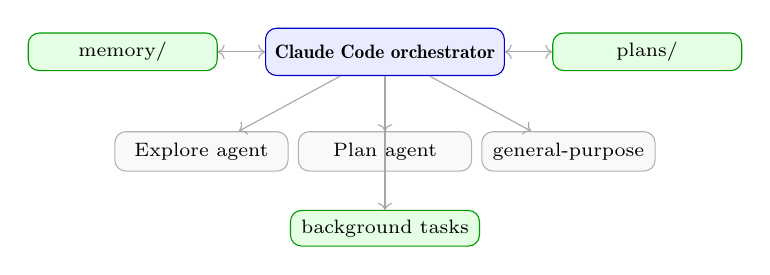
\begin{tikzpicture}[
    node distance=0.2cm,
    cc/.style={rectangle, rounded corners, draw=RedTitle, fill=blue!8,
        minimum width=3.0cm, minimum height=0.6cm, font=\scriptsize, text=DarkText, align=center},
    sub/.style={rectangle, rounded corners, draw=gray!60, fill=gray!5,
        minimum width=2.2cm, minimum height=0.5cm, font=\scriptsize, text=DarkText, align=center},
    disk/.style={rectangle, rounded corners, draw=green!60!black, fill=green!10,
        minimum width=2.4cm, minimum height=0.45cm, font=\scriptsize, text=DarkText, align=center}
]
\node[cc] (cc) {\textbf{Claude Code orchestrator}};
\node[sub, below left=0.7cm and -0.3cm of cc] (explore) {Explore agent};
\node[sub, below=0.7cm of cc] (plan) {Plan agent};
\node[sub, below right=0.7cm and -0.3cm of cc] (gen) {general-purpose};
\node[disk, left=0.6cm of cc] (memory) {memory/};
\node[disk, right=0.6cm of cc] (plans) {plans/};
\node[disk, below=1.7cm of cc] (bg) {background tasks};
\draw[->, gray!70] (cc) -- (explore);
\draw[->, gray!70] (cc) -- (plan);
\draw[->, gray!70] (cc) -- (gen);
\draw[<->, gray!70] (cc) -- (memory);
\draw[<->, gray!70] (cc) -- (plans);
\draw[->, gray!70] (cc) -- (bg);
\end{tikzpicture}
\end{center}
\end{column}
\begin{column}{0.42\textwidth}
\scriptsize
\textbf{What ran autonomously during the 8 weeks.}
\begin{itemize}\scriptsize
  \item \textbf{Plan mode.} Each stage drafted, edited, user-approved, executed. Plans live at \texttt{\~{}/.claude/plans/*.md} across sessions.
  \item \textbf{Sub-agents.} Explore agent spawned in parallel (sometimes 3 at once) to map the codebase before designing new scripts.
  \item \textbf{Memory.} Per-project files (\texttt{project\_*.md}, \texttt{MEMORY.md}) persisted what was done and where the track paused.
  \item \textbf{Background tasks.} Scripts 19 and 21b runs used \texttt{run\_in\_background} + \texttt{Monitor}, so planning continued while regressions compiled.
\end{itemize}
\end{column}
\end{columns}

\vspace{0.1cm}
\begin{tcolorbox}[colback=blue!3,colframe=RedTitle!60]\scriptsize
None of these were explicitly requested turn-by-turn. Claude Code \emph{chose} when to launch a sub-agent, when to save a memory, when to start a background task. The economist's job shifted from ``drive each step'' to ``approve each plan, critique each memo.''
\end{tcolorbox}
\end{frame}

% ============================================================
% Frame 5.42 --- Where custom agents/skills would help
% ============================================================
\begin{frame}{Where Reusable Skills Would Tighten the Loop}
\scriptsize
\begin{tabular}{p{3.0cm}p{4.4cm}p{4.6cm}}
\toprule
\textbf{Proposed skill} & \textbf{What it would do} & \textbf{Where it saves time} \\
\midrule
\texttt{index-builder} & Emit a new Script 2X with caching, z-scoring, and claims-discipline notes baked in. & Stage 1, 2, and 4 script scaffolding. \\
\texttt{regression-runner} & Given an outcome, features, and cells, emit the full F1--F5 regression ladder. & Stage 2 and Stage 4 regression boilerplate. \\
\texttt{label-corpus} & Wrap the bulk + adjudicate + cache pattern for large task-labeling jobs. & Turns similar corpus tasks into 1-day projects instead of 1-week projects. \\
\bottomrule
\end{tabular}

\vspace{0.16cm}
\begin{tcolorbox}[colback=blue!3,colframe=RedTitle!60]\scriptsize
\textbf{Interpretation.} The biggest gains now come from packaging repeated research patterns, not from asking the model to be smarter in a single conversation.
\end{tcolorbox}
\end{frame}

% ============================================================
% Frame 5.43 --- Reviewer / coordination agents
% ============================================================
\begin{frame}{Where Reviewer Agents Would Tighten the Loop}
\scriptsize
\begin{tabular}{p{3.0cm}p{4.4cm}p{4.6cm}}
\toprule
\textbf{Proposed agent} & \textbf{What it would do} & \textbf{Where it saves time} \\
\midrule
\texttt{memo-writer} & Enforce the six-element template on every end-of-stage memo and auto-link prior outputs. & Stage-close memos across the whole project. \\
\texttt{coauthor-critic} & Read the memo and surface the top missing checks, as a simulated reviewer. & Replaces part of the coauthor burden; never all of it. \\
\bottomrule
\end{tabular}

\vspace{0.16cm}
\begin{tcolorbox}[colback=blue!3,colframe=RedTitle!60]\scriptsize
\textbf{Claim.} Claude Code was already sufficient without custom tooling. The next 10$\times$ gain would come from making these repeated reviewer patterns reusable.
\end{tcolorbox}
\end{frame}

% ============================================================
% Frame 5.44 --- Three uses of LLMs
% ============================================================
\begin{frame}{The Power of LLMs in this Project --- Three Uses}
\begin{columns}[T]
\begin{column}{0.32\textwidth}
\textbf{1. LLM as pair programmer}
\begin{tcolorbox}[colback=gray!5,colframe=gray!40]\scriptsize
Writes Python, runs it, reads the output, iterates on user prompts. The entire pipeline (Scripts 01--30, 21b) falls here. Familiar from Cases 1--4.

\vspace{0.1cm}
Where it fires: every new script, every diagnostic, every figure.
\end{tcolorbox}
\end{column}
\begin{column}{0.32\textwidth}
\textbf{2. LLM as reviewer}
\begin{tcolorbox}[colback=gray!5,colframe=gray!40]\scriptsize
Critiques the empirical snapshot, proposes the next design. Stage 1's self-review memo (54 KB); the Apr 22 distillation of the coauthor critique into the Stage 4 question.

\vspace{0.1cm}
Where it fires: every end-of-stage frame in this deck.
\end{tcolorbox}
\end{column}
\begin{column}{0.32\textwidth}
\textbf{3. LLM as empirical data producer}
\begin{tcolorbox}[colback=blue!3,colframe=RedTitle!60]\scriptsize
Stage 3: per-task (e\_sub, e\_asst) labeling. 11,171 / 13,225 tasks labeled autonomously.

\vspace{0.1cm}
An LLM-labeled dataset of $10^4$ observations is a first-class empirical artifact --- versionable, cross-validatable, publishable.
\end{tcolorbox}
\end{column}
\end{columns}

\vspace{0.3cm}
\begin{tcolorbox}[colback=blue!3,colframe=RedTitle!60]\scriptsize
\textbf{The third use is the one most often missed.} A student who has only seen LLMs as writing assistants has not yet seen LLMs doing labor that was previously the province of thousands of MTurk workers or hundreds of RA-hours. That is the step change this case study is built around.
\end{tcolorbox}
\end{frame}

% ============================================================
% Frame 5.41 --- Ten Lessons (replaces Five Lessons)
% ============================================================
\begin{frame}{Ten Lessons from Case Study 5}
\scriptsize
\begin{columns}[T]
\begin{column}{0.48\textwidth}
\textit{From Stage 1 (first sprint):}
\begin{enumerate}\scriptsize
  \item \textbf{Lead with the puzzle, not the method.} First turn names what is unresolved; the method is downstream.
  \item \textbf{Empirics first buys theoretical honesty.} The data are the cheapest critic the theory will ever meet.
  \item \textbf{\texttt{config.py} + STOP GATES} = audit-grade pipeline: parameters on disk, inspections at named checkpoints.
  \item \textbf{When the interaction flips sign, audit the proxy before revising the theory.} A bad measure can imitate a broken mechanism.
  \item \textbf{A one-page snapshot} costs less than one rerun and compounds more than any single figure.
\end{enumerate}
\end{column}
\begin{column}{0.48\textwidth}
\textit{From Stages 2--4 (this extension):}
\begin{enumerate}\scriptsize
  \setcounter{enumi}{5}
  \item \textbf{The first sprint is never the last.} End-of-stage memos + honest coauthor critiques are the lowest-cost lever for the next sprint.
  \item \textbf{Orthogonality to $\bar E$ $\neq$ predictive power.} \texttt{top\_bottom\_gap} has $r^2$ on $\bar E$ of 0.001 but fires only in one cell. \texttt{task\_count} is correlated with $\bar E$ but wins the FRS horse race.
  \item \textbf{Joint F-tests understate power under multicollinearity.} Shapley R$^2$ decomposition separates collinear signal from noise.
  \item \textbf{LLMs are economically viable corpus labelers.} Bulk (Haiku) + adjudication (Sonnet) + per-task cache = 11k tasks labeled in one 5-h window.
  \item \textbf{Index design is scale-dependent.} \texttt{glue\_protection\_z} survives at Census 2018 but washes out at OCC1950 pooled. Declare the aggregation up-front.
\end{enumerate}
\end{column}
\end{columns}

\vspace{0.15cm}
\begin{tcolorbox}[colback=blue!3,colframe=RedTitle!60]\scriptsize
\textbf{Transferable pattern.} Replace ``glue work + AI labor market'' with any puzzle that has (i) a theoretical primitive, (ii) a public dataset, (iii) a visible post-event window, and (iv) a task corpus an LLM can score. The same four-stage scaffold runs on any of them.
\end{tcolorbox}
\end{frame}

%===========================================================
\section{Synthesis and Exercises}
%===========================================================

\sectiondivider{Synthesis and Exercises}{Comparing reusable skills, empirical pipelines, public-web datasets, and full-lifecycle collaboration}

\begin{frame}{Compare the Five Cases}
\scriptsize
\begin{tabular}{p{2.2cm}p{1.7cm}p{1.9cm}p{1.9cm}p{2.1cm}p{2.2cm}}
\toprule
 & \textbf{Case 1} & \textbf{Case 2} & \textbf{Case 3} & \textbf{Case 4} & \textbf{Case 5} \\
\midrule
Main artifact & review report & panel + figures & metadata dataset & repositioned paper & workflow walkthrough \\
Workflow type & reusable skill & 3-prompt session & batched public-web & full lifecycle collab. & meta / process audit \\
Main validation & quote accuracy & ext.\ benchmark & provenance & claims discipline & replayability on a new question \\
Main failure mode & hallucinated criticism & wrong crosswalk & weak sources & data-mining / sycophancy & pattern-matching to Case 4 instead of learning its method \\
\bottomrule
\end{tabular}
\end{frame}

\begin{frame}{When to Use Which Workflow}
\begin{columns}[T]
\begin{column}{0.24\textwidth}
\textbf{Build a skill}
\begin{itemize}\small
    \item repeated use
    \item high QC needs
    \item stable output format
\end{itemize}
\end{column}
\begin{column}{0.24\textwidth}
\textbf{Stay ad hoc}
\begin{itemize}\small
    \item one-off empirical job
    \item fast iteration
    \item small prompt set
\end{itemize}
\end{column}
\begin{column}{0.24\textwidth}
\textbf{Build a dataset harness}
\begin{itemize}\small
    \item many entities
    \item uneven sources
    \item provenance matters
\end{itemize}
\end{column}
\begin{column}{0.24\textwidth}
\textbf{Full-lifecycle collab.}
\begin{itemize}\small
    \item novel research question
    \item theory needs operationalization
    \item claims discipline required
    \item adversarial review needed
\end{itemize}
\end{column}
\end{columns}

\vspace{0.3cm}
\textbf{And Case 5?} Case 5 is not a fifth workflow to pick for a project. It is a meta-case: a walkthrough of Case 4's process so students can replay the same five-act scaffold on their own question. Pick Cases 1--4 to work; read Case 5 to learn how.
\end{frame}

\begin{frame}{The Division of Labor Across All Three}
\small
\begin{tabular}{p{5.9cm}p{6.0cm}}
\toprule
\textbf{Economist} & \textbf{Agent} \\
\midrule
define the question and success criteria & execute bounded tasks repeatedly \\
set the coding and validation rules & manipulate files, prompts, and reruns \\
spot implausible outputs & surface drafts, diagnostics, and plots \\
interpret the economic meaning & accelerate the path from question to artifact \\
\bottomrule
\end{tabular}

\vspace{0.3cm}
\textbf{The constant:} the question, the benchmark, and the interpretation remain human work.
\end{frame}

\begin{frame}{Failure Modes to Watch For}
\begin{enumerate}
    \item \textbf{Case 1:} confident but unsupported criticism
    \item \textbf{Case 2:} clean-looking code with a wrong variable mapping
    \item \textbf{Case 3:} a rich-looking dataset built on weak or forbidden sources
    \item \textbf{Case 4:} AI validates the design instead of challenging it, or data contradicts theory without adversarial structure to surface it
    \item \textbf{All cases:} hidden assumptions that never made it into project files
\end{enumerate}

\vspace{0.3cm}
\textbf{The cure is the same in all four cases:} name the validation step, save the rules on disk, and inspect the output like a referee.
\end{frame}

\begin{frame}{Exercises and Deliverables}
\small
\begin{tabular}{p{2.6cm}p{4.3cm}p{5.7cm}}
\toprule
\textbf{Exercise} & \textbf{Artifact} & \textbf{Deliverable} \\
\midrule
Exercise A: MEPS lab & harmonized panel and validated figures & in-class guided run with the existing notebook \\
Exercise B: fellows assignment & batch-level metadata dataset with provenance & normalized CSV, four figures, and a memo \\
\bottomrule
\end{tabular}

\vspace{0.3cm}
\begin{itemize}
    \item Exercise A teaches empirical execution and validation
    \item Exercise B teaches controlled public-web data construction
    \item Together they cover two distinct patterns students will actually face in research
\end{itemize}
\end{frame}

\begin{frame}{Looking Back at the Course}
\begin{center}
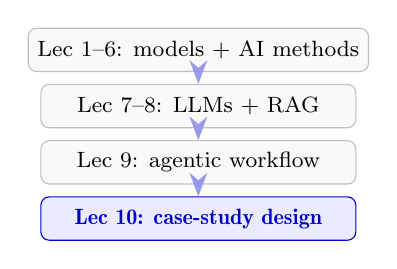
\begin{tikzpicture}[
    node distance=0.15cm,
    block/.style={rectangle, rounded corners=3pt, draw=gray!50, fill=gray!5,
        minimum width=4.0cm, minimum height=0.55cm, font=\footnotesize, text=DarkText},
    current/.style={rectangle, rounded corners=3pt, draw=RedTitle, fill=blue!8,
        minimum width=4.0cm, minimum height=0.55cm, font=\footnotesize\bfseries, text=RedTitle},
]
\node[block] (l12) {Lec 1--6: models + AI methods};
\node[block, below=of l12] (l78) {Lec 7--8: LLMs + RAG};
\node[block, below=of l78] (l9) {Lec 9: agentic workflow};
\node[current, below=of l9] (l10) {Lec 10: case-study design};

\draw[-{Stealth[length=3mm]}, thick, RedTitle!40] (l12.south) -- (l78.north);
\draw[-{Stealth[length=3mm]}, thick, RedTitle!40] (l78.south) -- (l9.north);
\draw[-{Stealth[length=3mm]}, thick, RedTitle!40] (l9.south) -- (l10.north);
\end{tikzpicture}
\end{center}

\vspace{0.2cm}
\textbf{Final message:} the distance from question to artifact has collapsed, but economists still own the standards for what counts as evidence.
\end{frame}

%===========================================================
% APPENDIX
%===========================================================

\appendix
\section{Appendix}

\sectiondivider{Appendix}{Operational details moved out of the main narrative}

\begin{frame}{Appendix A: Paper-Review Skill Internals}
\small
\begin{tabular}{lp{9.2cm}}
\toprule
\textbf{Component} & \textbf{Role} \\
\midrule
\texttt{SKILL.md} & orchestrates the 7-phase pipeline \\
\texttt{shared-directives.md} & confidence gate, tone, quote rules \\
\texttt{section-prompts.md} & specialized prompts by section type \\
\texttt{editorial-prompt.md} & final quality gate before output \\
\bottomrule
\end{tabular}

\vspace{0.3cm}
\textbf{Reason this is appendix material:} students need to understand the workflow design before they need a file inventory.
\end{frame}

\begin{frame}[fragile]{Appendix B: MEPS Prompt Skeleton}
\begin{lstlisting}[style=pythonstyle, language={}, basicstyle=\ttfamily\scriptsize, numbers=none]
Prompt A: download + parse + harmonize + save panel
Prompt B: compute weighted rates by year and subgroup
Prompt C: generate annotated publication-quality figures
\end{lstlisting}

\vspace{0.25cm}
\textbf{Operational note:} the notebook remains the handout for the in-class lab.
\end{frame}

\begin{frame}{Appendix C: Fellows Normalized Schema}
\small
\begin{tabular}{p{3.6cm}p{8.1cm}}
\toprule
\textbf{Column group} & \textbf{Examples} \\
\midrule
seed fields & name, affiliation, election year \\
source fields & official profile URL, bio URL, CV URL \\
biography fields & birth date raw, birth year, PhD year, gender explicit \\
research fields & research fields raw, normalized field bucket \\
audit fields & source\_birth, source\_phd, source\_gender, source\_field, notes \\
\bottomrule
\end{tabular}
\end{frame}

\begin{frame}{Appendix D: Fellows Batching Rule}
\begin{itemize}
    \item official roster parsed into 18 batches of 50
    \item students complete one batch at a time
    \item every batch must report coverage before interpretation
    \item if birth-year coverage stays low, use years since PhD instead of age
\end{itemize}
\end{frame}

\begin{frame}{Appendix E: Resources}
\begin{itemize}
    \item Lecture 10 MEPS notebook in this folder
    \item \texttt{Exercise10\_ES\_Fellows/} script bundle in this folder
    \item Official Econometric Society current fellows page, checked April 13, 2026
    \item MEPS public-use files and external benchmark sources used in Case Study 2
\end{itemize}
\end{frame}

\end{document}
